\chapter{The DUNE Near Detector} % Executive Summary}
\label{ch:exsum-nd}

\textit{This chapter briefly introduces the DUNE near detector, emphasizing its role for the DUNE far detector physics program.  More details on the near detector may be found in  appendices of this TDR volume.  DUNE will issue a complete conceptual design report for the near detector in late 2019, with a technical design report to follow in 2020.}

%%%%%%%%%%%%%%%%%%%%%%%%%%%%%%%%%%%%%%%%%%%%%%%%%%%%%%%%%%%%%%
\section{Overview of the DUNE Near Detector}
\label{sec:exsum-nd-overview}


\subsection{Motivation}
\label{sec:exsum-nd-BriefOverview-need}

This chapter briefly summarizes the purpose and reference design concept for the \dword{dune} \dword{nd}.  A more complete description may be found in the appendices of this volume.

The \dword{dune} experiment is intended to measure oscillation probabilities for muon neutrinos or antineutrinos to either remain the same flavor or oscillate into their electron flavor counterparts as a function of the neutrino energy. This will allow the neutrino mass ordering to be definitively determined, as well as enable observation of leptonic \dword{cpv} for a significant range of $\delta_{\rm{CP}}$ values and precise measurement of % \dword{pmns}
neutrino mixing matrix parameters.

The \dword{nd} will serve as the experiment's control,
 constraining systematic errors and measuring the initial unoscillated \numu and \nue energy spectra. %The energy spectrum is a convolution of three functions: the neutrino flux as a function of energy and species; neutrino-nucleus cross sections as a function of energy, reaction type, and event kinematics (e.g., 4-momentum transfer); and the detector response.
 The energy spectra result from an energy-dependent convolution of flux, cross section, and detector response for each of the four neutrino types.
  The \dword{nd} will make measurements that allow the three functions to be independently constrained and partially or fully deconvolved. The constraints will be used to improve the simulation program that is responsible for predicting the energy spectra at the \dword{fd} for particular choices of the oscillation parameters. This allows the actual oscillation parameters to be estimated from a fit to the \dword{fd} data. 
 
% To first order, a far/near ratio (or migration matrix), derived from the simulation, can predict the unoscillated energy spectrum at the \dword{fd} based on the \dword{nd} measurements.  The energy spectra at the \dword{fd} are then sensitive to the oscillation parameters, which can be extracted via a fit. 

%The \dword{nd} must have as many methods for measuring neutrino fluxes as possible. independent of cross section uncertainties. The need to rely on models means the \dword{nd} must measure neutrino interactions with much higher detail than the \dword{fd}.  It must also be able to measure events much like the \dword{fd} does, so it can determine the ramifications of the more limited \dword{fd} performance, provide corrections, and take advantage, to some extent, of effects cancelling in the near-to-far extrapolation.

The \dword{nd} will also have a physics program of its own, independent of the far detector.  This program will include measuring neutrino interactions to explore the two pillars of the standard model: electroweak physics and quantum chromodynamics. The \dword{nd} physics program will also explore physics beyond the standard model. This includes searches for non-standard interactions, sterile neutrinos,  dark photons, and  other exotic particles.

 %%%%%%%%%%%%%%%%%%%%%%%%%
\subsection{Requirements}
\label{sec:exsum-nd-requirements}

%As discussed in Sections~\ref{sec:exsum-nd-role} and \ref{sec:exsum-nd-overview}, the \dword{dune}  \dword{nd} complex has many missions, and 
The components of the  \dword{nd} must address their multiple missions in a complementary fashion. In this section, we list the key overarching requirements driving the \dword{nd} complex. Section~\ref{sec:appx-nd:requirements} in Appendix~\ref{ch:appx-nd} goes into more detail, discussing some thought experiments and case studies that illustrate how different parts of the complex work together. These case studies naturally suggest more detailed capabilities, performance statistics, and technical requirements; we are in the process of tabulating them. 

\begin{itemize}
    \item  \textit{Predict the neutrino spectrum at the \dword{fd}} The \dword{nd} must predict the energy spectrum of \numu, \anumu, \nue and \anue at the \dword{fd}. The prediction must be provided as a function of the oscillation parameters, and systematic uncertainties must be small enough to achieve the required \dword{cp} coverage. This is the primary requirement of the \dword{dune} \dword{nd}.
    
    \item \textit{Measure interactions on argon} The \dword{nd} must measure neutrino interactions on argon to reduce uncertainties due to nuclear modeling. The \dword{nd} must be able to determine the neutrino flavor and measure the full kinematic range of the interactions that will be seen at the \dword{fd}.
    
    \item \textit{Measure the neutrino energy} The \dword{nd} must be able to reconstruct the neutrino energy in \dword{cc} events and control for any biases in energy scale or resolution, keeping them small enough to achieve the required \dword{cp} coverage. These measurements must also be transferable to the \dword{fd}. 
    
    \item \textit{Constrain the cross section model} The \dword{nd} must measure neutrino cross sections in order to constrain the cross section model used in the oscillation analysis. In particular, cross section mismodeling that causes incorrect \dword{fd} predictions as a function of neutrino flavor and true or reconstructed energy must be constrained well enough to achieve the required \dword{cp} coverage. 
    
    \item \textit{Measure neutrino fluxes} The \dword{nd} must measure neutrino fluxes as a function of flavor and neutrino energy. This allows neutrino cross section to be measured and constrains the beam model and the extrapolation of neutrino energy spectra from the \dword{nd} to the \dword{fd}.
    
    \item \textit{Obtain data with different fluxes} The \dword{nd} must measure neutrino interactions in different beam fluxes (especially ones with different mean energies) to disentangle flux and cross sections, verify the beam model, and guard against systematic uncertainties on the neutrino energy reconstruction.
    
    \item \textit{Monitor the neutrino beam} The \dword{nd} must monitor the neutrino beam energy spectrum with sufficient statistics to be sensitive to intentional or accidental changes in the beam on short timescales. The precise requirement will be informed by the run plan and by experience from previous experiments. 
    
\end{itemize}


\subsection{Design}
\label{sec:exsum-nd-BriefOverview-design}

% MK: I don't think this is needed. 
%The conceptual design of the \dword{dune}  \dword{nd} uses the collective experience of the many \dword{dune} collaborators who have participated significantly in the current generation of neutrino experiments. 

The \dword{dune} \dword{nd} is formed from three primary detector components and the capability of two of those components to move off the beam axis. The three detector components serve important individual and overlapping functions in the \dword{nd} mission.  Because these components have standalone features, the \dword{dune} \dword{nd} is often discussed as a suite or complex of detectors and capabilities.  The movement off axis provides a valuable extra degree of freedom in the data, which is discussed extensively in this report.  The power in the \dword{dune} \dword{nd} concept lies in the collective set of capabilities.  

The \dword{dune} \dword{nd} is shown in the \dword{dune} \dword{nd} hall in Figure~\ref{fig:es:NDHallconfigs}.  Table~\ref{tab:es:NDsumm} provides a high-level overview of the three components of the \dword{dune} \dword{nd} along with the off-axis capability that is sometimes described as a fourth component.  

\begin{dunefigure}[DUNE near detector hall with component detectors]{fig:es:NDHallconfigs}
{\dword{dune} \dword{nd} hall shown with component detectors, all in the on-axis configuration (left) and with the \dword{lartpc} and \dword{mpd} in an off-axis configuration (right). The \dword{3dsts} is shown in position on the beam axis. The beam axis is also shown.  The beam enters the hall at the bottom of the drawings moving from right to left.}
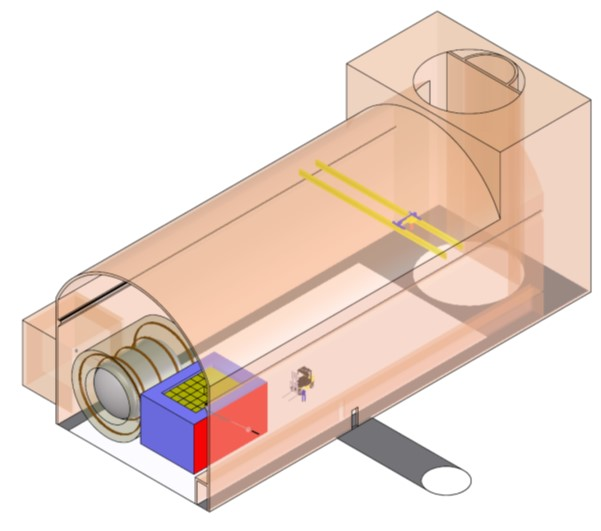
\includegraphics[width=0.49\textwidth]{graphics/NDHall_onaxis.jpg}
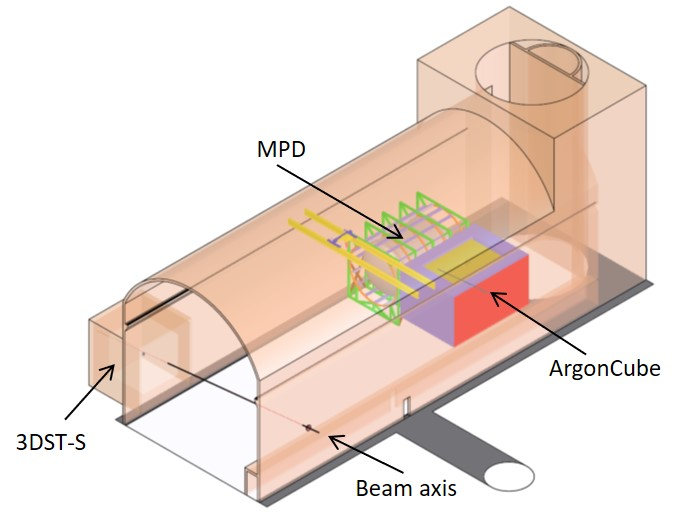
\includegraphics[width=0.49\textwidth]{graphics/NDHall_offaxis.jpg}
\end{dunefigure}



\begin{dunetable}[Components of the DUNE ND]
{p{.22\textwidth}p{.22\textwidth}p{.22\textwidth}p{.22\textwidth}}
{tab:es:NDsumm}{This table gives a high-level breakdown of the three major detector components and the capability of movement for the DUNE ND along with function and primary physics goals.}
Component & Essential Characteristics & Primary function & Select physics aims \\ \toprowrule
LArTPC (ArgonCube) & Mass  & Experimental control for the FD & $\numu$($\overline{\nu}_{\mu}$) CC \\
          & Target nucleus Ar &  Measure unoscillated $E_\nu$ spectra   & $\nu$-e$^{-}$ scattering   \\
          &  Technology FD-like    &  Flux determination  &  $\nue +$$\overline{\nu}_{e}$ CC  \\
          &  &  &  Interaction model \\ \colhline
Multipurpose detector (MPD) & Magnetic field & Experimental control for the LArTPCs & $\numu$($\overline{\nu}_{\mu}$) CC \\
  &  Target nucleus Ar & Momentum analyze liquid Ar $\mu$ & $\nue$ CC, $\overline{\nu}_{e}$ \\
  & Low density & Measure exclusive final states with low momentum threshold & Interaction model \\  \colhline
DUNE-PRISM & LArTPC$+$MPD move off-axis & Change flux spectrum &  
Deconvolve flux$\times$cross section \\ 
 & & & Energy response \\
 & & & Provide FD-like energy spectrum at ND\\ 
% & & & {\   }differences \\
 & & & ID mismodeling \\ \colhline
\dword{3dsts} & On-axis & Beam flux monitor &  On-axis flux stability \\ 
  & Mass & Neutrons & Interaction model \\ 
& Magnetic field &  & A dependence \\
    & CH target & & $\nu$-e$^{-}$ scattering \\ 
\end{dunetable}


The core part of the \dword{dune} \dword{nd} is a \dword{lartpc} called \dword{arcube}.  \dword{arcube} consists of an array of 35 modular \dwords{tpc} sharing a cryostat.  A drawing of a prototype of the modular \dwords{tpc} is illustrated in Figure~\ref{fig:es:ac_module}.  %The particular implementation of the \dword{lartpc} technology in this detector is described in Section~\ref{sec:exsum-nd-lartpc} below.  
This detector has the same target nucleus and shares some aspects of form and functionality with the \dword{fd}, where the differences are necessitated by the expected intensity of the beam at the \dword{nd}.  This similarity in target nucleus and, to some extent, technology, reduces sensitivity to nuclear effects and detector-driven systematic errors in the extraction of the oscillation signal at the  \dword{fd}.  The \dword{lartpc} is large enough to provide high statistics ($\num{1e8}{\numu \text{-CC events/year}}$) and sufficient volume to provide good hadron containment.  The tracking and energy resolution, combined with the mass of the \dword{lartpc}, will allow the flux in the beam to be measured using several techniques, including the well understood but rare process of $\nu$-e$^{-}$ scattering.

\begin{dunefigure}[ArgonCube 2$\times$2 demonstrator module]{fig:es:ac_module}
{Cutaway drawing of a \SI{0.67 x 0.67 x 1.81}{\metre} \dword{arcube} prototype module. For illustrative purposes, the drawing shows traditional field shaping rings instead of a resistive field shell. Note the G10 walls will completely seal the module, isolating it from the neighboring modules and the outer \dword{lar} bath. Also note the modules in this prototype system will not have individual pumps and filters.}
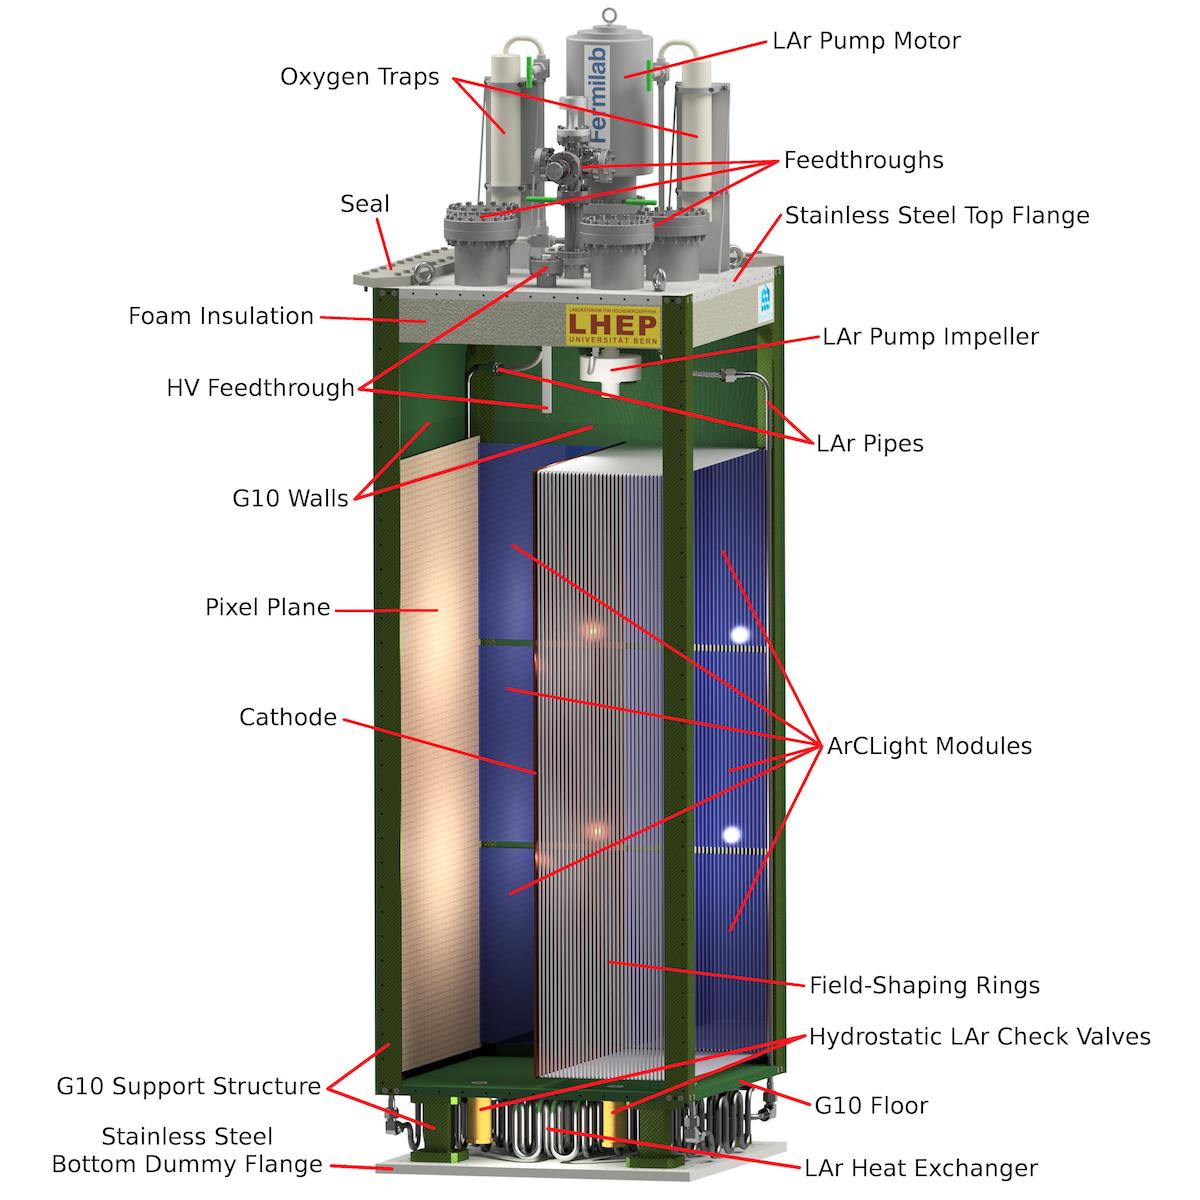
\includegraphics[width=0.8\textwidth]{graphics/Normal-Module-4K_labelled.jpeg}
\end{dunefigure}

The \dword{lartpc} begins to lose acceptance for muons above 0.7 GeV/c momentum due to lack of containment.  Because the muon momentum is a critical component of the neutrino energy determination, a magnetic spectrometer is needed downstream of the \dword{lartpc} to measure the charge sign and momentum of these muons.  This function is accomplished by the multipurpose detector (\dword{mpd}), which consists of a high-pressure gaseous argon \dword{tpc} (\dword{hpgtpc}) surrounded by an \dword{ecal} in a \SI{0.5}{T} magnetic field. See Figures~\ref{fig:es:ConceptDesign_NDECAL} and~\ref{fig:es:ConceptTile_NDECAL}. 
The \dword{hpgtpc} provides a lower density medium with excellent tracking resolution for the muons from the \dword{lartpc}.  In addition, with this choice of technology for the tracker, neutrinos interacting on the argon in the gas \dword{tpc} constitute a sample of $\nu$-Ar events that can be studied with a very low charged particle tracking threshold, excellent kinematic resolution, and systematic errors that differ from the liquid detector. The high pressure results in a sample of $\num{2e6}$ ${\numu \text{-CC events/year}}$ for these studies. These events will be valuable for studying the charged particle activity near the interaction vertex because this detector can access lower momentum protons than the \dword{lar} detector and has better particle identification of charged $\pi$'s.  The relative reduction in secondary interactions in these samples (compared to \dword{lar}) will help in identifying the particles produced in the primary interaction and modeling secondary interactions in denser detectors, which are known to be important \cite{Friedland:2018vry}.
In addition, many neutrons produced in neutrino interactions in the gaseous argon may be reconstructed via time-of-flight using the \dword{ecal}.    
  
%The \dword{mpd} is  discussed further in Section~\ref{ssec:exsum-nd-mpd}.

\begin{dunefigure}[\dshort{mpd} ECAL conceptual design]{fig:es:ConceptDesign_NDECAL}
{On the left, the conceptual design of the HPgTPC + \dword{ecal} barrel system for the \dword{nd}. In the preliminary design, the full \dword{ecal} is located inside the HPgTPC pressure vessel. On the right, a conceptual design of the \dword{ecal} endcap system.}
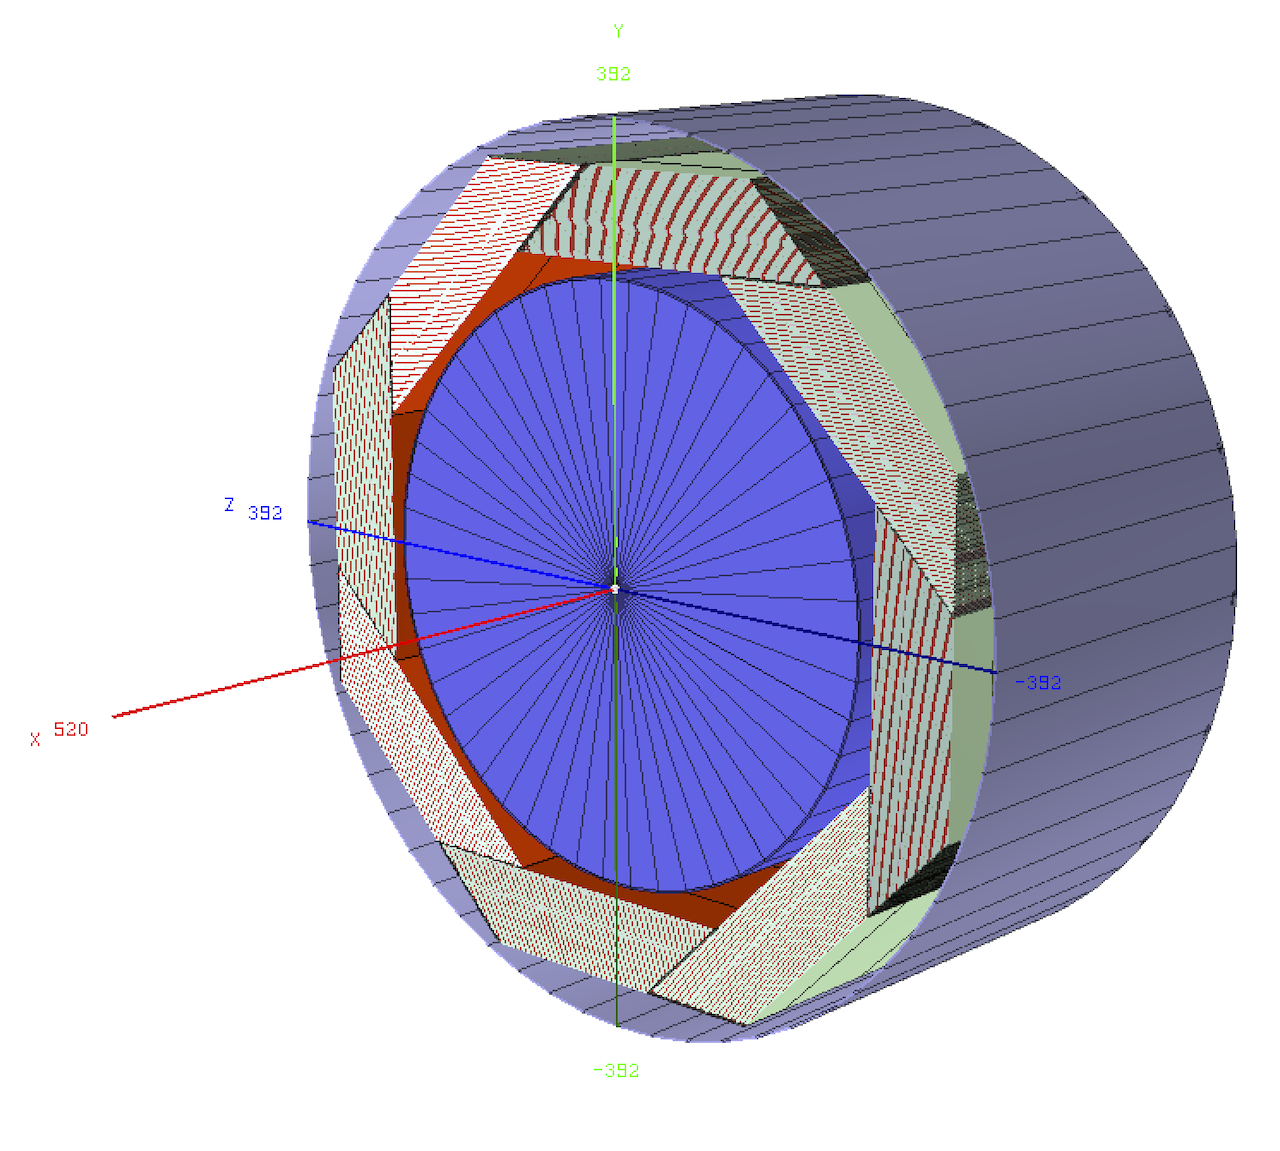
\includegraphics[width=0.45\textwidth]{graphics/ConceptECALND.png}
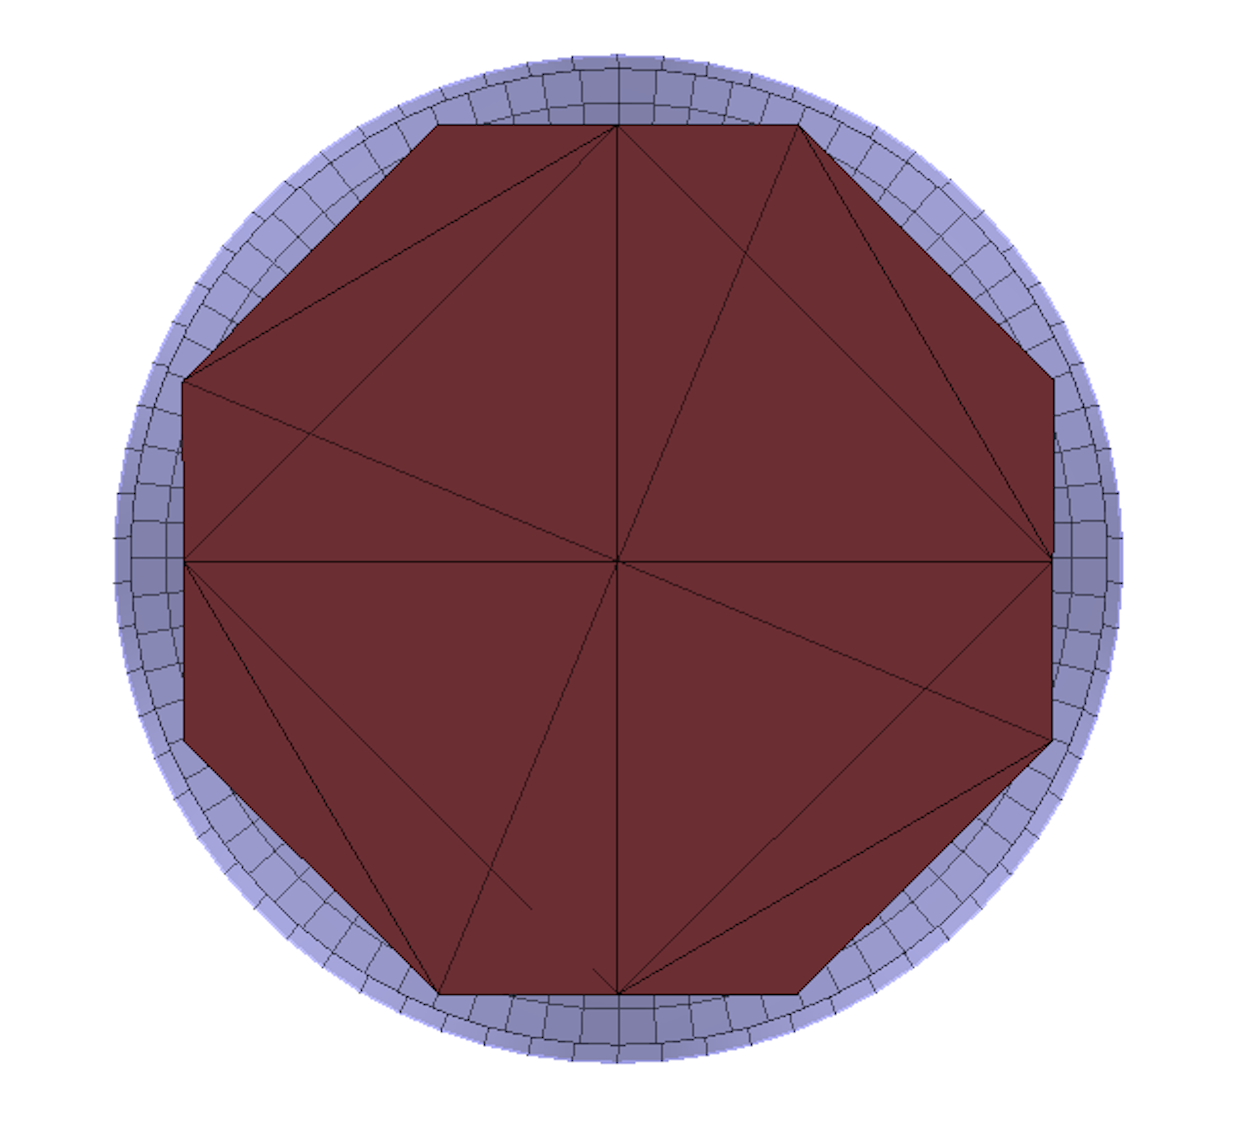
\includegraphics[width=0.42\textwidth]{graphics/ECAL_Endcap_System.png}
\end{dunefigure}

\begin{dunefigure}[Conceptual layout of the \dshort{mpd} ECAL]{fig:es:ConceptTile_NDECAL}
{Conceptual layout of the calorimeter showing the absorber structure, scintillator tiles, \dword{sipm}, and \dword{pcb}. The scintillating layers consist of a mix of tiles and cross-strips with embedded wavelength shifting fibers to achieve a comparable effective granularity.}
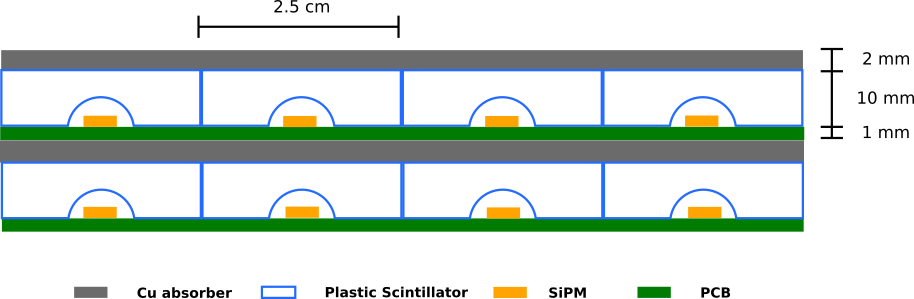
\includegraphics[width=0.8\textwidth]{graphics/TileConcept.png}
\end{dunefigure}

The \dword{lartpc} and \dword{mpd} can move to take data in positions off the beam axis.  This capability is referred to as \dword{duneprism}. As the detectors move off-axis, the incident neutrino flux spectrum changes, with the mean energy dropping and the spectrum becoming more monochromatic.  Though the neutrino interaction rate drops off-axis, the intensity of the beam and the size of the \dword{lartpc}  combine to yield ample statistics even in the off-axis positions. 
Figure~\ref{fig:es:offaxisfluxes} shows a sample of neutrino energy distributions taken at different off-axis angles.
%
Data taken at different off-axis angles allows the deconvolution of the neutrino flux and interaction cross section and mapping of the reconstructed versus true energy response of the detector.  This latter mapping is applicable at the \dword{fd} up to the level to which the near and far \dword{lar} detectors are similar.  Stated a different way, it is possible to use information from a linear combination of the different fluxes to create a data sample at the \dword{nd} with an effective neutrino energy distribution close to the oscillated spectrum at the \dword{fd}.  This data-driven technique will reduce systematic effects coming from differences in the energy spectra of the oscillated signal events in the \dword{fd} and the \dword{nd} samples used to constrain the interaction model. Finally, the off-axis degree of freedom provides a sensitivity to some forms of mismodeling in the beam and/or interaction models. %The \dword{duneprism} program is discussed further in Section~\ref{sec:exsum-nd-DP}. 
Figure~\ref{fig:es:duneprismfluxfits} shows linear combinations of off-axis fluxes giving \dword{fd} oscillated spectra for two sets of oscillation parameters. 

%\fixme{This shows up in the PDF as an incomplete sentence. What shows?}

%%%
\begin{dunefigure}[Variation of neutrino energy spectrum as function of off-axis angle]{fig:es:offaxisfluxes}
{The variation in the neutrino energy spectrum shown as a function of detector off-axis position, assuming the nominal \dword{nd} location 574~m downstream from the production target.}
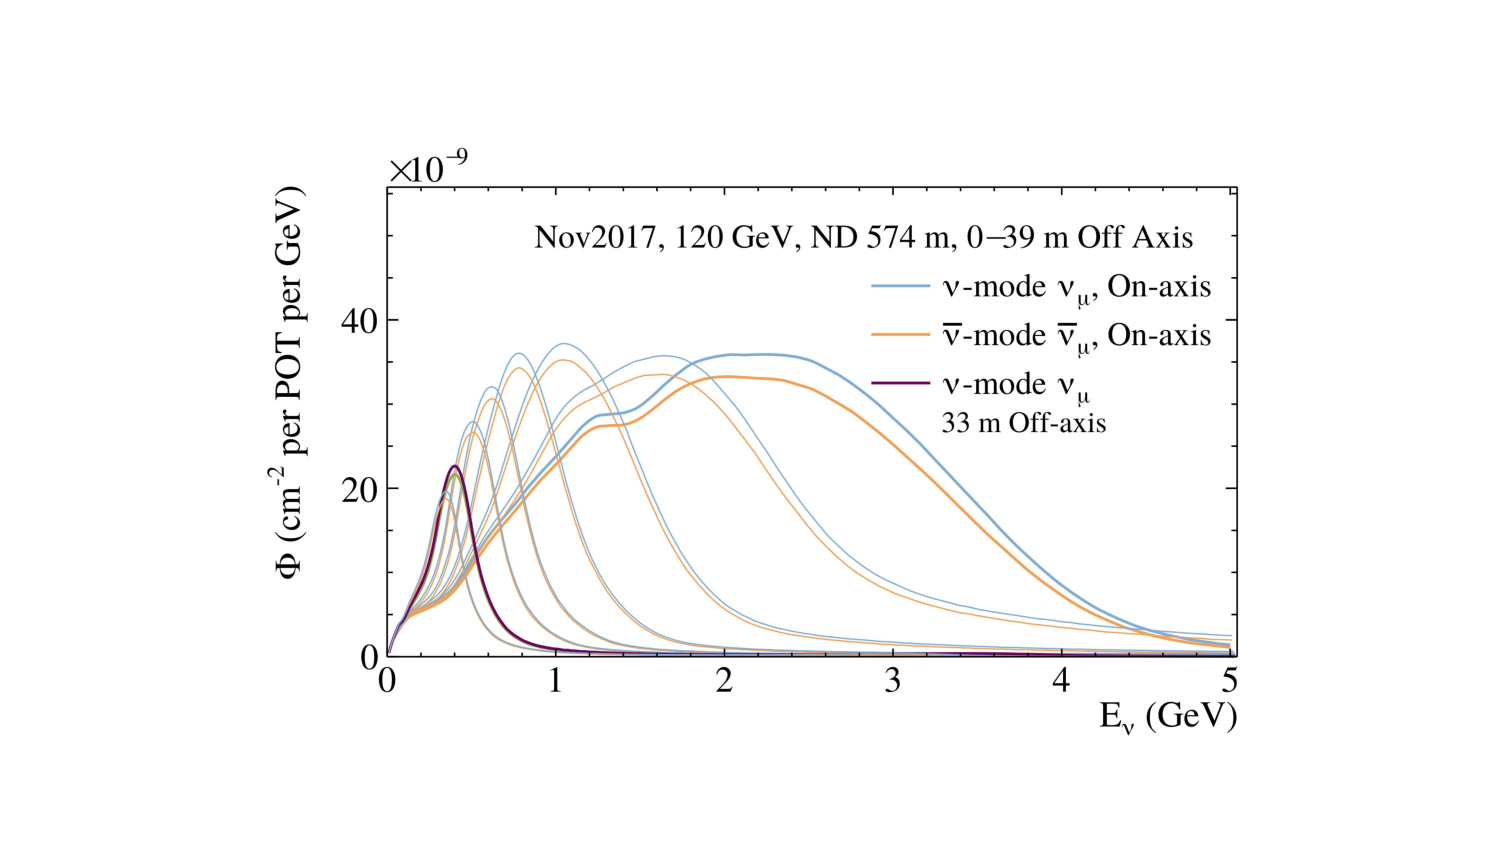
\includegraphics[width=0.8\textwidth]{offaxisfluxes.pdf}
\end{dunefigure}
%%
\begin{dunefigure}[Linear combinations of off-axis fluxes giving FD oscillated spectra]{fig:es:duneprismfluxfits}
{Linear combinations of off-axis fluxes giving \dword{fd} oscillated spectra for a range of oscillation parameters. The  \dword{fd} oscillated flux is shown in black, the target flux is shown in green, and the linearly combined flux obtained with the nominal beam \dword{mc} is shown in red. Systematic effects due to 1$\,\sigma$ variations of the decay pipe radius (green), horn current (magenta), and horn cooling water layer thickness (teal) are also shown.}
	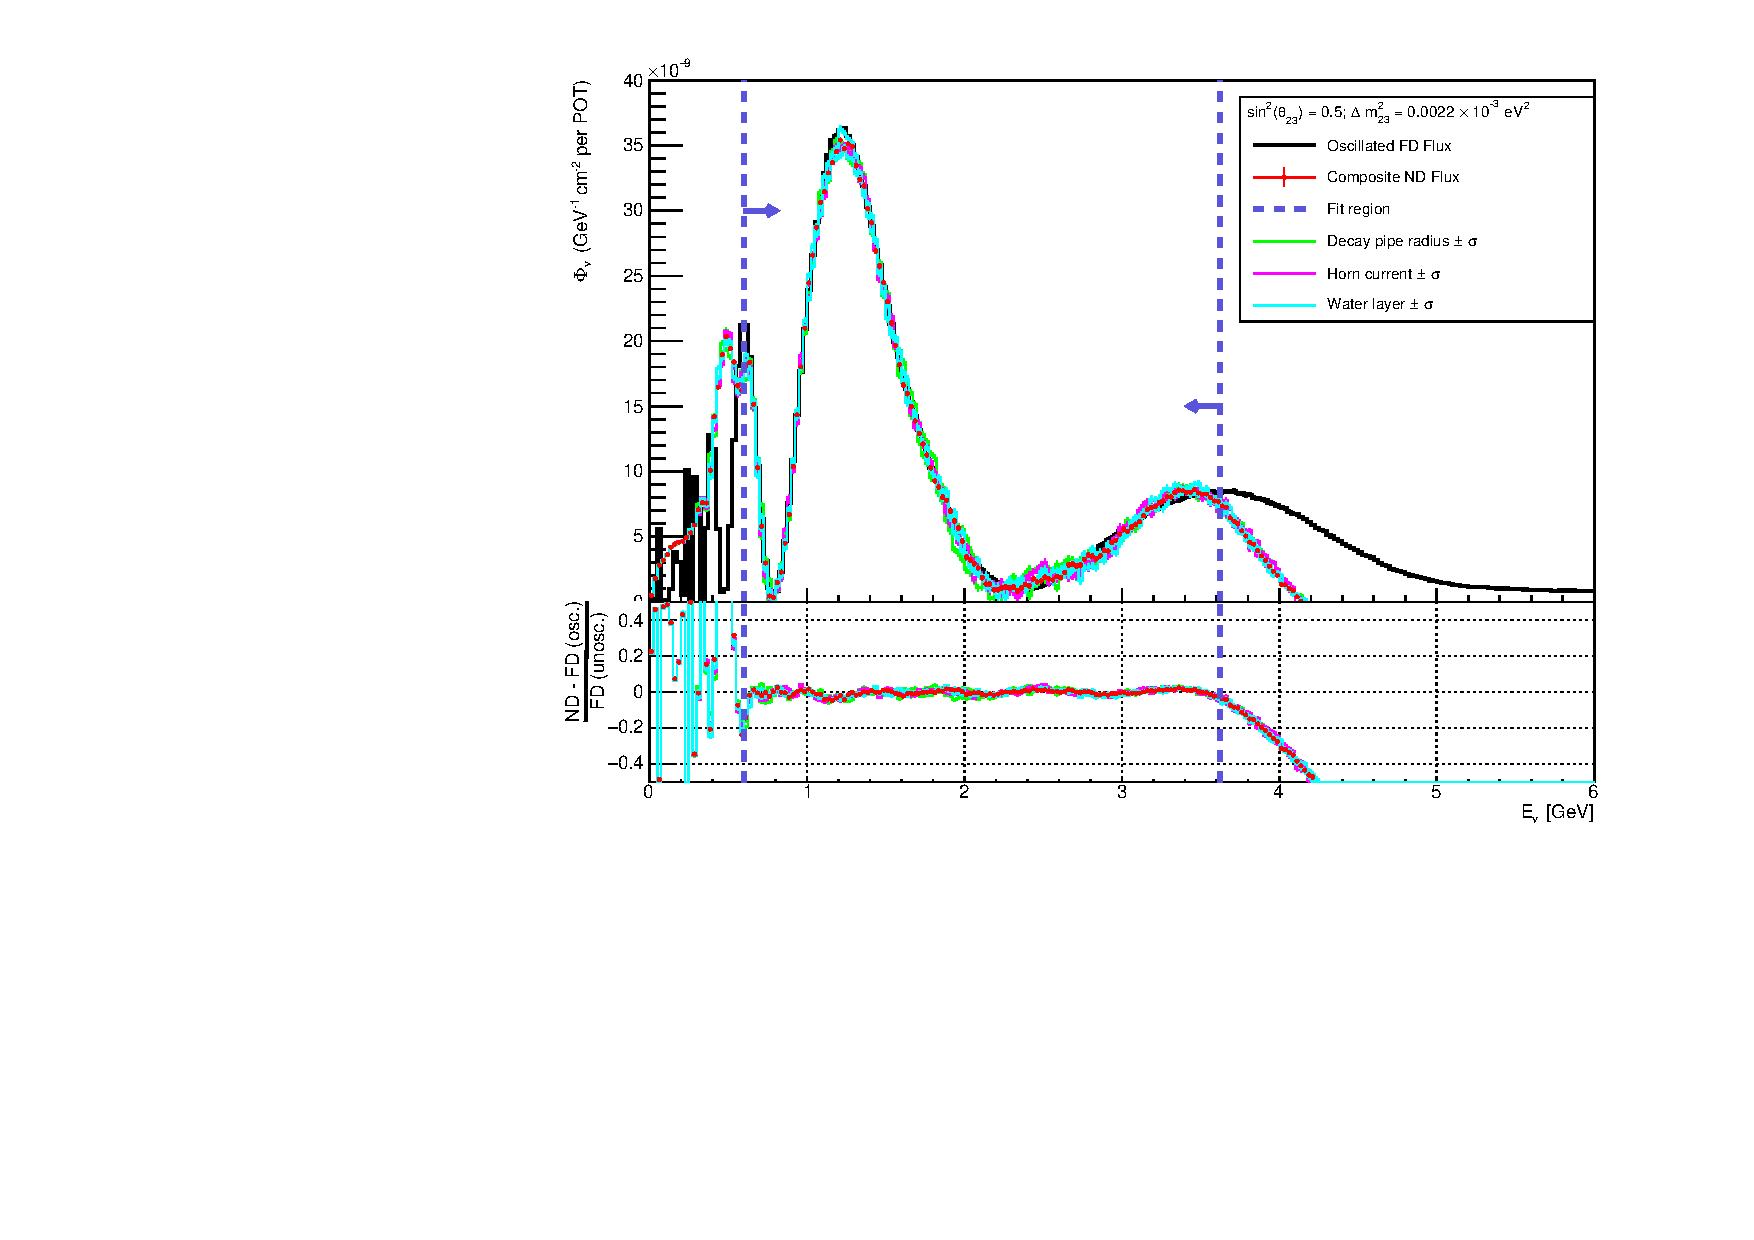
\includegraphics[width=0.7\textwidth]{nuprism_coef_oscSpectrum_0_0022_0_5.pdf}
	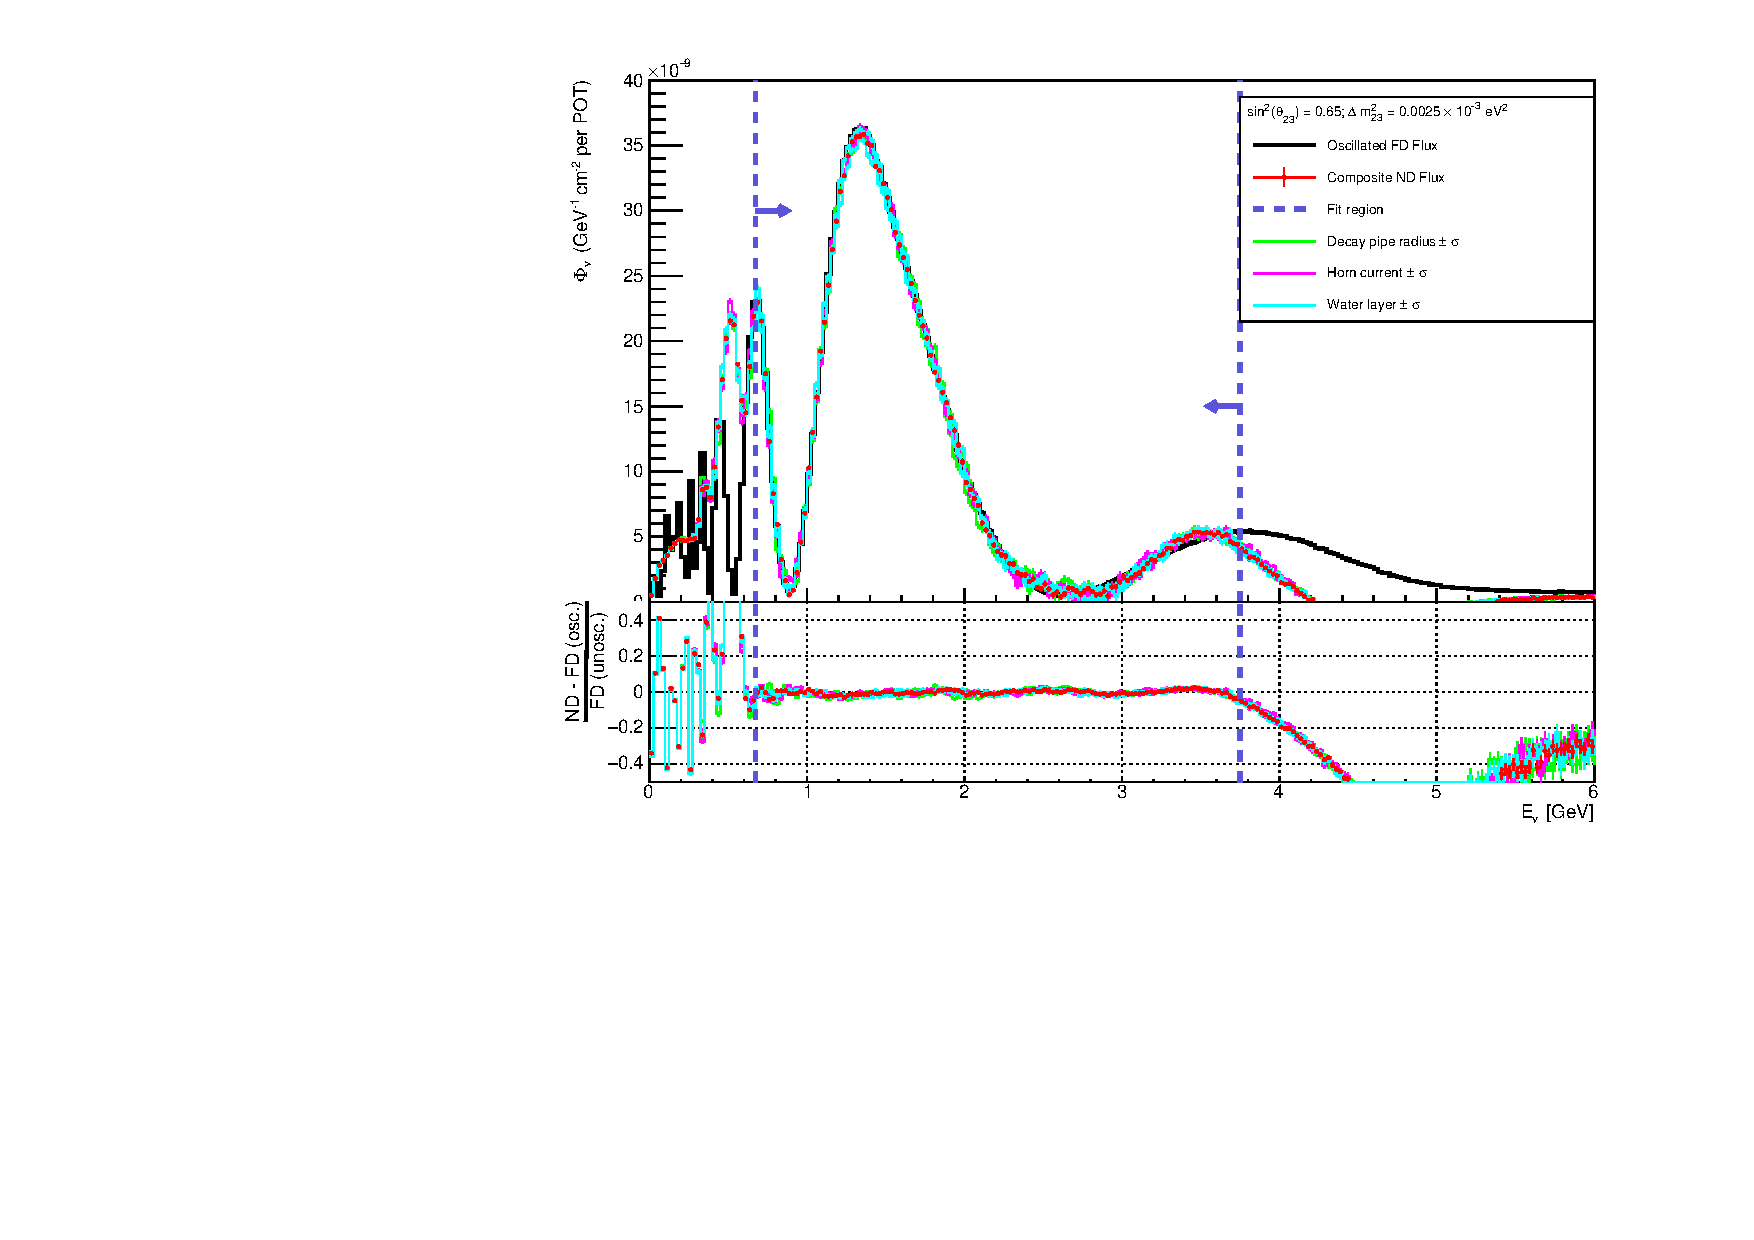
\includegraphics[width=0.7\textwidth]{nuprism_coef_oscSpectrum_0_0025_0_65.pdf}
\end{dunefigure}
%%

The final component of the \dword{dune} \dword{nd} suite is the \threed projection scintillator tracker spectrometer (\dword{3dsts}),  the core part of which is the \dword{3dst}, as illustrated in Figure~\ref{fig:es:3dst-geometry}.  The \dword{3dst} is a plastic scintillator detector made of \SI{1}{\cubic\centi\meter} cubes read out along each of three orthogonal dimensions.  The design eliminates the typical planar-strip geometry common to detectors using a scintillator, leading to improved acceptance at large angles relative to the beam direction.  The \dword{3dst} is situated along the beam axis inside an envelope of high resolution, normal pressure \dwords{tpc} and an \dword{ecal}.  The entire structure is enclosed in a magnet. This device serves as a dedicated  neutrino spectrum monitor that stays on-axis when the   \dword{lartpc} and \dword{mpd} have moved to an off-axis position. 
It also provides an excellent on-axis, neutrino flux determination using many of the methods discussed in Appendix~\ref{sec:appx-nd:fluxappendix}. The neutrino flux determined using this detector, with  differing detectors, targets, and interaction systematic errors from the \dword{lartpc}, is an important point of comparison and a systematic crosscheck for the flux as determined by the \dword{lartpc}.

\begin{dunefigure}[The \dshort{3dsts} detector configuration]{fig:es:3dst-geometry}
{The \dword{3dsts} detector configuration, including the \dword{3dst} (blue), \dwords{tpc} (orange), \dword{ecal} (green), and the magnet (purple).}
  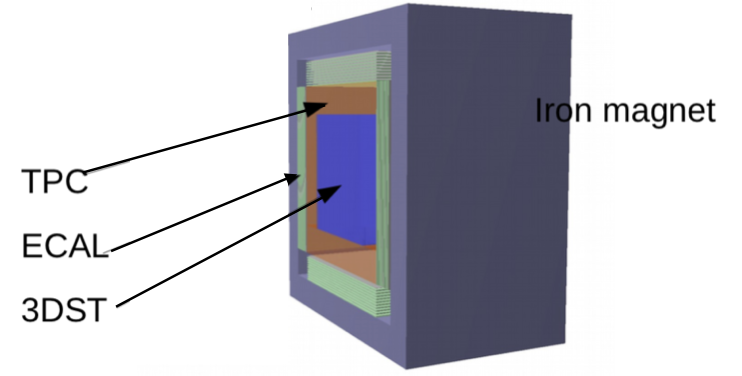
\includegraphics[width=7.in]{3dst-geometry.png}
\end{dunefigure}




In addition, the \dword{3dst} has very fast timing and can isolate small energy depositions from neutrons in three dimensions.  This provides the capability to  incorporate neutrons in the event reconstruction using energy determination via time-of-flight with a high efficiency. This capability should be useful for the low-$\nu$ flux determination because it allows events to be tagged with a significant neutron energy component or provides a way to include that energy in the calculation.  Including neutrons in detailed studies of neutrino interactions in the \dword{3dsts} using single transverse variables may prove useful in motivating improvements in the neutrino interaction model. Although the target for this device is carbon, not argon, basic insights into components of the interaction model may extend to argon.  For example, the multinucleon component of the interaction model will be used for argon although it was developed in response to observations made on plastic targets.   



\section{Role of the ND in the DUNE Oscillation Program}
\label{sec:exsum-nd-role}

Oscillation experiments must accomplish three main tasks. First, they must identify the flavor of interacting neutrinos in \dword{cc} events or identify the events as \dword{nc} interactions. Second, they must measure the energy of the neutrinos because oscillations occur as a function of baseline length over neutrino energy, \dword{l/e}. Third, they must compare the observed event spectrum in the \dword{fd} to  predictions based on differing sets of oscillation parameters, subject to constraints from data observed in the \dword{nd}.  That comparison and how it varies with the oscillation parameters allows oscillation parameters to be measured.

The connection between the observations in the \dword{nd} and the \dword{fd} is made using a simulation that convolves models of the neutrino flux, neutrino interactions, nuclear effects, and detector response.
This gives rise to a host of complicating effects that 
muddy the simple picture. They come from two main sources. First, the identification efficiency is not \SI{100}{\%}, and there are
some background events (for example, \dword{nc} with a $\pi^0$ are a background to \nue \dword{cc} interactions). Both the efficiency and background are imperfectly known. %Generally, it is helpful to have a  \dword{nd} that is as similar as feasible to the  \dword{fd} because a bias in the efficiency as a function of energy will cancel between the two detectors. 
Because the background level tends to be similar in both the \dword{fd} and \dword{nd}, it helps if the \dword{nd} can characterize backgrounds better than the \dword{fd}. %, either due to its technology, or by leveraging the much larger statistics and freedom to take data in alternative beam configuration modes (for example, different horn currents or movement off the beam axis). 
%

The second major source of complication occurs because the \dword{fd} (and the similar \dword{nd}) must be made of heavy nuclei rather than hydrogen. %Neutrino interactions can be idealized as a three stage process: (1) a neutrino impinges on a nucleus with nucleons in some initial state configuration, (2) scattering occurs with one of the nucleons, perhaps creating mesons, and (3) the hadrons reinteract with the remnant nucleus on their way out (so called \dwords{fsi}). 
The presence of the nucleus affects %all three stages 
neutrino interactions in ways that ultimately drive the design of the  \dword{nd} complex. In particular, in a detector with heavy nuclei the nucleons in the initial state of the nucleus are mutually interacting and exhibiting Fermi motion. Neutrinos therefore interact with moving nucleon targets. The wavelength of the interaction varies with momentum transfer but is often long enough to simultaneously probe multiple nucleons. Another complication is that neutrino cross sections on {\em free nucleons} are not generally well known in the kinematic range interesting for \dword{dune}, but neutrino-nucleus scattering models rely on these neutrino-nucleus cross sections. A final complication comes about because neutrinos produce hadrons with the nucleus itself. After production the hadrons undergo \dword{fsi} and are thereby attenuated as they leave the target nucleus. Section~\ref{sec:appx-nd:exsum-nd-role} of Appendix~\ref{ch:appx-nd} discusses neutrino nucleus scattering in more detail. The \dword{dune} \dword{nd} includes liquid and gaseous active targets that will make high statistics measurements on argon, rather than another nucleus, to reduce nuclear model dependence. 


Neutrons can be produced from the struck nucleus, as well as from follow-on interactions of the neutrino's reaction-products with other nuclei. The energy carried away by neutrons is difficult to detect and can bias the reconstructed neutrino energy. The \dword{3dst} and \dword{mpd} have capabilities that allow neutron energy to be directly measured. The \dword{duneprism} program constrains the true to reconstructed energy relation and is thus also sensitive to energy carried by neutrons.

Heavy nuclei in the detector offer additional complications for particles that have left the struck nucleus, especially in the case where the detector is dense, as is the case for the \dword{lartpc}. Particles produced in a neutrino interaction may  reinteract inside the detector, creating electromagnetic and hadronic cascades. These cascades, particularly the hadronic ones, degrade the detector's performance. They confuse the reconstruction program due to overlapping energy and event features. They also result in a degredation of the energy resolution and result in additional energy carried by neutrons that may go missing. Particle identification by $dE/dx$ is also less effective for early showering particles. In addition, low-energy particle tracks in a dense detector may be too short to detect.  The \dword{dune} \dword{nd} includes the \dword{mpd} with a \dword{gartpc} that allows neutrino interactions to be measured on argon but with significantly fewer secondary interactions and much lower energy tracking thresholds.



Finally, setting aside complications due to heavy nuclei and dense detectors, we note that a significant fraction of the neutrino interactions in \dword{dune} will come from inelastic processes, not the simpler \dword{qe} scattering. 
This typically leads to a more complex morphology for events and greater challenges for the detector and the modeling.  The \dword{dune} \dword{nd} acts as a control for the \dword{fd} and is designed to be more capable than the \dword{fd} at measuring complicated inelastic events.

The complexity described above is incorporated imperfectly into the neutrino interaction model. The predicted signal in the \dword{nd} is a convolution of this interaction model with the beam model and the detector response model.  The critical role of  the  \dword{nd} is to supply the observations used to tune, or calibrate, this convolved model, thereby reducing the overall uncertainty in the expected signal at the \dword{fd} which is used for extracting the oscillation parameters via comparison with the observed signal.  Additionally, with the high statistics and very capable subsystems, the \dword{nd} data sets provide the raw material used to improve the models beyond simple tuning.  


%%%%%%%%%%%%%%%%%%%%%%%%%%%%%%%%%%%%%%%%%%%%%%%%%%%%%%%%%%%%%%
\section{ND Hall and Construction}
\label{sec:exsum-nd-hall}
%% \chapter defined in lbne-sci-opp-main.tex

The DUNE near neutrino detector provides scientific value beyond
      its essential role of calibrating beam and neutrino interaction
      properties for the long-baseline physics program described in
      Chapter~\ref{nu-oscil-chap}.
      By virtue of the theoretically clean, purely weak leptonic
      processes involved,
      neutrino beams have historically served as unique probes for
      new physics in their interactions with matter.
      The high intensity and broad energy range of the LBNF beam
      will open the door for a highly capable near detector
      to perform its own diverse
program of incisive investigations. 

%\fixme{Simplified this pgraph a bit per Jim's wish to make the ND seem less optional}
The reduction of systematic uncertainties for the neutrino oscillation
program %of the full DUNE scope requires a highly capable near neutrino detector (ND) to provide 
requires excellent resolution in the
reconstruction of neutrino events. Combined with the unprecedented
neutrino fluxes available %for the DUNE program 
--- which will
allow the collection of ${\cal{O}}$(\num{e8}) inclusive neutrino charged
current (CC) interactions for %\SI{e22}{\POT} 
\num{e22} protons-on-target (POT) just downstream of the
beamline --- the %inclusion of a 
near detector (ND)  %offers a unique opportunity to 
will significantly enhance the DUNE long-baseline 
oscillation program and produce a range of short-baseline neutrino
scattering physics measurements.  The combined statistics and
resolution expected in the ND will allow precise tests of fundamental
interactions resulting in a better understanding of the structure of
matter. 
Table~\ref{tab:rates} lists the expected number of %muon neutrino
beam-neutrino interactions per ton of detector at the DUNE ND site,
located \SI{459}{\meter} downstream from
the %beginning of the decay pipe
target.  
% \fixme{check this sentence; and the table 7.1 caption says
% 'interactions in the beams' (which is weird) and is for a water
% detector. Is this what you want?}  MB: interactions in the neutrino
% beam are interactions in the near detector when the neutrino beam is
% shining on it.  the calculations were made for water. leave as is
This chapter presents a short description of some of the studies that
can be performed with DUNE's fine-grained near neutrino detector
and gives a flavor of the outstanding physics potential. A more
detailed and complete discussion of the ND physics
potential can be found in~\cite{docdb-6704}.
Appendix~\ref{app-dis} describes neutrino scattering 
kinematics and includes
definitions of the kinematic variables used in this chapter.
\begin{table}[!htb]
\centering
\caption[Interaction rates, $\nu$ mode, per ton
for \SI{1e20}{\POT}, \SI{459}{\meter}, \SI{120}{\GeV}]{Estimated interaction rates in the neutrino (second column) and antineutrino (third column) beams per ton of detector (water) 
  for \SI{1e20}{\POT} at \SI{459}{\meter} assuming neutrino
  cross-section predictions from NUANCE~\cite{Casper:2002sd} and a \GeVadj{120}
  proton beam using the CDR reference design.  Processes are defined at the initial neutrino
  interaction vertex and thus do not include final-state effects. These estimates do not
  include detector efficiencies or acceptance~\cite{DOCDB740,DOCDB783}. 
}
\label{tab:rates}
\begin{tabular}[!htbp]{$L^r^r}%rl}  %$
\toprule
\rowtitlestyle
Production mode & $\nu_\mu$ Events & $\overline\nu_\mu$ Events\\
\toprowrule
CC QE ($\nu_\mu n \rightarrow \mu^- p$)                             & 50,100 & 26,300 \\ \colhline
NC elastic ($\nu_\mu N \rightarrow \nu_\mu N$)                      & 18,800 & 8,980 \\ \colhline
CC resonant $\pi^+$ ($\nu_\mu N \rightarrow \mu^- N \pi^+$)         & 67,800 & 0 \\ \colhline
CC resonant $\pi^-$ ($\overline{\nu}_\mu N \rightarrow \mu^+ N \pi^-$)   & 0      & 20,760 \\ \colhline
CC resonant $\pi^0$ ($\nu_\mu n \rightarrow \mu^- \ p \, \pi^0$)    & 16,200 & 6,700 \\ \colhline
NC resonant $\pi^0$ ($\nu_\mu N \rightarrow \nu_\mu \, N \, \pi^0$) & 16,300 & 7,130 \\ \colhline
NC resonant $\pi^+$ ($\nu_\mu p \rightarrow \nu_\mu \, n \, \pi^+$) & 6,930  & 3,200 \\ \colhline
NC resonant $\pi^-$ ($\nu_\mu n \rightarrow \nu_\mu \, p \, \pi^-$) & 5,980  & 2,570 \\ \colhline
CC DIS ($\nu_\mu N \rightarrow \mu^- X$ or 
$\overline{\nu}_\mu N \rightarrow \mu^+ X$, $W>2$)                     & 66,800 & 13,470 \\ \colhline
NC DIS ($\nu_\mu N \rightarrow \nu_\mu X$ or 
$\overline{\nu}_\mu N \rightarrow \overline{\nu}_\mu X$, $W>2$)                   & 24,100 & 5,560 \\ \colhline
NC coherent $\pi^0$ ($\nu_\mu A \rightarrow \nu_\mu A \pi^0$ or 
$\overline{\nu}_\mu A \rightarrow \overline{\nu}_\mu A \pi^0$
)       & 2,040  & 1,530 \\
CC coherent $\pi^+$ ($\nu_\mu A \rightarrow \mu^- A \pi^+$)         & 3,920  &  0 \\ \colhline
CC coherent $\pi^-$ ($\overline{\nu}_\mu A \rightarrow \mu^+ A \pi^-$)   & 0      & 2,900 \\ \colhline
NC resonant radiative decay ($N^* \rightarrow N \gamma $)          & 110    & 50 \\ \colhline
%Cabbibo-suppressed QE hyperon production & & \\ \colhline
%($\mu^+ \Lambda, \mu^+ \Sigma^0, \mu^+ \Sigma^-$) & 0 & xxx  \\ \colhline
NC elastic electron ($\nu_\mu e^- \rightarrow \nu_\mu e^-$  
or  $\overline{\nu}_\mu e^- \rightarrow \overline{\nu_\mu} e^-$)              & 30  & 17 \\ \colhline
Inverse Muon Decay ($\nu_\mu e \rightarrow \mu^- \nu_e$)            & 12  & 0\\ \colhline
Other                                                              & 42,600 & 15,800 \\ 
\toprule
\rowtitlestyle
Total CC  (rounded)                                                       & 236,000 & 81,000 \\ %81,340 \\
\rowtitlestyle
Total NC+CC  (rounded)                                                      & 322,000 & 115,000 \\%114,980 \\ 
\bottomrule
\end{tabular}
\end{table}
%%%%%%%%%%%%%%%%%%%%%%%%%%%%%%%%%%%%%%%%%%%%%%%%%%%%%%%%%%%%%%%%%%%%
\section{Precision Measurements with Long-Baseline Oscillations}
\label{sec-fluxosc}
From the studies of uncertainties and the impact of the spectral shape
presented in Section~\ref{sec:systs}, it is evident that to fully
realize the goals of the full DUNE scientific program --- in
particular, sensitivity to CP violation and the precision measurement
of the three-flavor oscillation parameters --- it is necessary to
characterize the expected unoscillated neutrino flux with high
precision. In addition to the precise determination of the neutrino
flux, shape and flavor composition, the characterization of different
neutrino interactions and interaction cross sections on a liquid argon target
is necessary to estimate physics backgrounds to the oscillation
measurements.  The high-resolution near tracking detector %such as that
described in Section~\ref{sec:ndproj} can measure the unoscillated flux
normalization, shape and flavor to a few percent using systematically
independent techniques that are %listed here and 
discussed in the following sections.
%%%%%%%%%%%%%%%%%%%%%%%%%%%%%%%%%%%%%%
\subsection{Determination of the Relative Neutrino and Antineutrino Flux} 
\label{sec-lownu0}
The most promising method of determining the shape of the \numu and
\anumu flux is by measuring CC events with low 
hadronic-energy deposition (low-$\nu$) where $\nu$ is the total energy of the
hadrons that are produced after a neutrino interaction, $E_\nu -
E_\mu$. It is important to note that not all the hadrons escape the
remnant nucleus, and intranuclear effects will smear the visible energy
of the hadronic system.  A method of relative flux determination known
as low-$\nu_0$ --- where $\nu_0$ is a given value of visible hadronic
energy in the interaction that is selected to minimize the fraction of
the total interaction energy carried by the hadronic system
--- is well developed~\cite{srmishra-reviewtalk}.  The method follows
from the general expression of the $\nu$-nucleon differential cross
section:
\begin{equation}
{\cal N} (\nu < \nu_0) \simeq C \Phi(E_\nu) \nu_0 \left[ {\cal A} +
\left( \frac{\nu_0}{E_\nu} \right) {\cal B} + \left( \frac{\nu_0}{E_\nu} \right)^2 {\cal C} +
{\cal O} \left( \frac{\nu_0}{E_\nu} \right)^3 \right],
\end{equation}
\noindent
where the coefficients are ${\cal A} = {\cal F}_2$, ${\cal B} = ({\cal
  F}_2 \pm {\cal F}_3)/2$, ${\cal C} = ({\cal F}_2 \mp {\cal F}_3)/6$, 
and ${\cal F}_i =\int^1_0 \int^{\nu_0}_0 F_i(x) dx d\nu$ is the
integral of structure function $F_i(x)$.  
%
The dynamics of
neutrino-nucleon scattering  implies that the number of events in a
given energy bin with hadronic energy $E_{\rm had} < \nu_0$ is
proportional to the (anti)neutrino flux in that energy bin up
to corrections ${\cal O}(\nu_0/E_\nu)$ and ${\cal O}(\nu_0/E_\nu)^2$.
%
The number ${\cal
  N}(\nu<\nu_0)$ is therefore proportional to the flux up to correction factors
of the order ${\cal O} (\nu_0/E_\nu)$ or smaller, which are not
significant for small values of $\nu_0$ at energies $\geq \nu_0$. 
 The coefficients ${\cal A}$, ${\cal B}$ and ${\cal C}$ are
determined for each energy bin and neutrino flavor within the ND data.
DUNE's primary interest is the relative flux
determination, i.e., the neutrino flux in one energy bin relative to that in
another; variations in the coefficients do not affect the
relative flux. The prescription for the relative flux determination is
simple: count the number of %$\nu$ 
neutrino CC events below a certain small
value of hadronic energy ($\nu_0$).  The observed number of events, up
to the correction of the order ${\cal O} (\nu_0/E_\nu)$ due to the
finite $\nu_0$ in each total visible energy bin, is proportional to
the relative flux. The smaller the factor $\nu_0/E_\nu$ is, the smaller
is the correction.  Furthermore, the energy of events passing the
low-$\nu_0$ cut is dominated by the corresponding lepton energy. 
It is
apparent from the above discussion that this method of relative flux
determination is not very sensitive to nucleon structure, QCD
corrections or types of neutrino interactions such as scaling or
nonscaling. With the excellent granularity and resolution foreseen in
the low-density magnetized tracker, it will be possible to use a value
of $\nu_0\sim$\SI{0.5}{\GeV} or lower, thus allowing flux predictions down to
$E_\nu \sim$\SI{0.5}{\GeV}. A preliminary analysis with the high-resolution
tracker achieved a precision $\leq 2\%$ on the relative $\nu_\mu$
flux with the low-$\nu_0$ method in the energy region $1 \leq E_\nu
\leq 30$ \si{GeV} in the fit with $\nu_0 < 0.5$ \si{\GeV}. Similar uncertainties
are expected for the $\overline{\nu}_\mu$ component (the dominant one) in
the antineutrino beam mode (negative focusing).
%%%%%%%%%%%%%%%%%%%%%%%%%%%%%%%%%%%%%%
\subsection{Determination of the Flavor Content of the Beam} 
%$\boldsymbol{\nu_\mu, \overline{\nu}_\mu, \nu_e, \overline{\nu}_e}$}
$\boldsymbol{\numu,\anumu, \nue, \anue}$
\fixme{I can't get this to compile with it in the heading. Anne}
The empirical parameterization %(EP)
of the pion and kaon neutrino parents produced from the proton target,
determined from the low-$\nu_0$ flux at the ND, allows prediction of
the $\nu_\mu$ and $\overline{\nu}_\mu$ flux at the far detector
location.  This parameterization provides a measure of the
$\pi^+/K^+/\mu^+(\pi^-/K^-/\mu^-)$ distributions of neutrino parents
of the beam observed in the ND.  Additionally, with the capability to
identify $\overline{\nu}_e$ CC interactions, it is possible to
directly extract the elusive $K^0_L$ content of the beam.  Therefore,
an accurate measurement of the $\nu_\mu, \overline{\nu}_\mu$ and
$\overline{\nu}_e$ CC interactions provides a prediction of the
$\nu_e$ content of the beam, which is an irreducible background for
the $\nu_e$ appearance search in the far detector:
\begin{eqnarray} \label{eqn:nueparents}
\nu_e & \equiv & \mu^+(\pi^+\to \nu_\mu) \oplus K^+(K^+\to \nu_\mu) \oplus K^0_L\\
\overline{\nu}_e & \equiv & \mu^-(\pi^-\to \overline{\nu}_\mu) \oplus K^-(K^-\to \overline{\nu}_\mu) \oplus K^0_L
\end{eqnarray}
The $\mu$ component is well constrained from $\nu_\mu
(\overline{\nu}_\mu)$ CC data at low energy, while the $K^\pm$
component is only partially constrained by the $\nu_\mu
(\overline{\nu}_\mu)$ CC data at high energy and requires external
hadro-production measurements of $K^\pm/\pi^\pm$ ratios at low energy
from hadro-production experiments such as MIPP~\cite{Raja:2005sh} and
NA61~\cite{Korzenev:2013gia}.  Finally, the $K_L^0$ component can be
constrained by the $\overline{\nu}_e$ CC data and by external
dedicated measurements at hadron-production experiments.  In the
energy range $1 (5) \leq E_\nu \leq 5 (15)$ \si{GeV}, the approximate
relative contributions to the $\nu_e$ spectrum are 85\% (55\%) from
$\mu^+$, 10\% (30\%) from $K^+$ and 3\% (15\%) from $K_L^0$.
Based on the NOMAD experience, %we expect to achieve
a precision of $\leq 0.1\%$ on the flux ratio $\nu_e/\nu_\mu$ is
expected at high energies. Taking into account the projected precision
of the $\nu_\mu$ flux discussed in Section~\ref{sec-lownu0}, this
translates into an absolute prediction for the $\nu_e$ flux at the
level of $2\%$.
Finally, the fine-grained ND can directly identify $\nu_e$ CC
interactions from the LBNF beam. The relevance of this measurement is
twofold:
\begin{enumerate}
\item It provides an independent
validation for the flux predictions obtained from the low-$\nu_0$ method.
\item It can
further constrain the uncertainty on the knowledge of the absolute $\nu_e$ flux.
\end{enumerate}
%%%%%%%%%%%%%%%%%%%%%%%%%%%%%%%%%%%%%%
\subsection{Constraining the Unoscillated $\nu$ %$\boldsymbol{\nu}$ 
Spectral Shape with the QE Interaction}
\fixme{took out bold -won't compile. Anne}

In any long-baseline neutrino oscillation program, including DUNE, the
quasi-elastic (QE) interactions are special.  First, the QE cross
section is substantial at lower energies~\cite{Formaggio:2013kya}.
Second, because of the simple topology (a $\mu^-$ and a proton), the
visible interaction energy provides, to first order, a close
approximation to the neutrino energy ($E_\nu$).  
In the context of a fine-grained tracker, a precise measurement of QE
will impose direct constraints on nuclear effects related to both the
primary and final-state interaction (FSI) dynamics 
(Section~\ref{sec-nuclear}), which can affect the overall neutrino
energy scale and, thus, the entire oscillation program.  To this end,
the key to reconstructing a high-quality sample of $\nu_\mu$ QE
interactions is the two-track topology where both final-state
particles are visible: $\mu^-$ and $p$. A high-resolution ND can
efficiently identify the recoil proton and measure its momentum vector
as well as $dE/dx$. Preliminary studies indicate that in a
fine-grained tracking detector the efficiency (purity) for the proton
reconstruction in QE events is $52\%$ ($82\%$). A comparison between
the neutrino energy reconstructed from the muon momentum through the
QE kinematics (assuming a free target nucleon) with the visible
neutrino energy measured as the sum of $\mu$ and $p$ energies is
sensitive to both nuclear effects and FSI. Furthermore, comparing the
two-track sample ($\mu$ and $p$) with the single-track sample (in which only $\mu$
is reconstructed) empirically constrains the rate of FSI.
%%%%%%%%%%%%%%%%%%%%%%%%%%%%%%%%%%%%%%
\subsection{Low-Energy Absolute Flux: Neutrino-Electron NC Scattering}
\label{ssec:ncscatter}
Neutrino neutral current (NC) interaction with the atomic electron in the
target, $\nu_\mu e^- \rightarrow \nu_\mu e^-$, provides an elegant
measure of the absolute flux.  The total cross section for NC elastic
scattering off electrons is given by~\cite{Marciano:2003eq}:
\begin{eqnarray}
\sigma (\nu_l e \to \nu_l e) & = & \frac{G_\mu^2 m_e E_\nu}{2\pi} \left[ 1 -4 \sin^2 \theta_W + \frac{16}{3} \sin^4 \theta_W \right], \\
\sigma (\overline{\nu}_l e \to \overline{\nu}_l e) & = & \frac{G_\mu^2 m_e E_\nu}{2\pi} \left[ \frac{1}{3} -\frac{4}{3} \sin^2 \theta_W + \frac{16}{3} \sin^4 \theta_W \right], 
\end{eqnarray}
\noindent
where $\theta_W$ is the weak mixing angle (WMA).  For the currently
known value of $\sin^2 \theta_W\simeq0.23$, the above cross sections
are very small: $\sim 10^{-42} (E_\nu/{\rm GeV})$~cm$^2$. The NC
elastic scattering off electrons can be used to determine the absolute
flux normalization since the cross section only depends on the
knowledge of $\sin^2 \theta_W$. Within the Standard Model, the value
of $\sin^2 \theta_W$ at the average momentum transfer expected at
DUNE, $Q\sim0.07$~\si{\GeV}, can be extrapolated down from the
LEP/SLC\footnote{LEP was the Large Electron-Positron Collider at CERN
  that operated from 1989 to 2000 and provided a detailed study of the
  electroweak interaction.}  measurements with a precision of $\leq
1\%$. The \numu $e^- \rightarrow$ \numu $e^-$ will produce a single
$e^-$ collinear with the $\nu$-beam ($\leq 40$~mrad).  The background,
dominated by the asymmetric conversion of a photon in an ordinary
$\nu$-nucleon NC event, will produce $e^-$ and $e^+$ in equal measure
with much broader angular distribution.  A preliminary analysis of the
expected elastic scattering signal in the high-resolution tracking ND
shows that the scattering signal can be selected with an efficiency of
about 60\% with a small background contaminant. The measurement will
be dominated by the statistical error. %We estimate that
The determination of the absolute flux of the DUNE neutrinos is
estimated to reach a precision of $\simeq 2.5\%$ for $E_\nu \leq
10$~\si{\GeV}.  The measurement of NC elastic scattering off electrons
can only provide the integral of all neutrino flavors.
%%%%%%%%%%%%%%%%%%%%%%%%%%%%%%%%%%%%%%
\subsection{High-Energy Absolute Flux: Neutrino-Electron CC Scattering}
The \numu-$e^-$ CC interaction, \numu$ + e^- \rightarrow \mu^- +
$\nue (\emph{inverse muon decay} or \emph{IMD}), offers an elegant
way to determine the absolute flux. Given the energy threshold needed
for this process, IMD requires %a minimum
$E_\nu \geq 10.8$~\si{\GeV}.  The high-resolution ND in the
LBNF beam will observe $\geq$ \num{2000} IMD events in three
years. The reconstruction efficiency of the single, energetic %and
forward $\mu^-$ will be $\geq$ 98\%; the angular resolution of the
IMD $\mu$ is $\leq$ \SI{1}{\mrad}. The background, primarily from the
$\nu_\mu$-QE interactions, can be precisely constrained using control
samples.  In particular, the systematic limitations of the CCFR
(\cite{Mishra:1989jn,Mishra:1990yf}) and %those of
the CHARM-II~\cite{Vilain:1996yf} IMD measurements can be
substantially alleviated in DUNE with the proposed ND design. A
preliminary analysis indicates that the absolute flux can be
determined with an accuracy of $\approx 3\%$ for $E_\nu \geq$
\SI{11}{\GeV} (average $E_\nu \approx$\SI{25}{\GeV}).
%%%%%%%%%%%%%%%%%%%%%%%%%%%%%%%%%%%%%%
\subsection{Low-Energy Absolute Flux: QE in Water and Heavy-Water Targets}
Another  % third 
independent method to extract the absolute flux is through the
QE-CC scattering ($\nu_\mu n(p) \to \mu^- p(n)$) on
deuterium at low $Q^2$. Neglecting terms in $(m_\mu/M_n)^2$ at $Q^2=0$,
the QE cross section is independent of neutrino energy for $(2E_\nu
M_n)^{1/2} > m_\mu$:
\begin{equation}
\frac{d \sigma}{d Q^2}  \mid {Q^2=0}\mid = \frac{G_\mu^2 \cos^2 \theta_c}{2\pi}
\left[ F_1^2(0) + G_A^2(0) \right] = 2.08 \times 10^{-38}~\rm cm^2{\rm GeV}^{-2},
\end{equation}
%
\noindent 
which is determined by neutron $\beta$ decay and has a theoretical
uncertainty $<1\%$.  The flux can be extracted experimentally by
measuring low $Q^2$ QE interactions ($ \leq 0.05$ GeV) and extrapolating
the result to the limit of $Q^2=0$. The measurement requires a
deuterium (or hydrogen for antineutrino) target to minimize the
smearing due to Fermi motion and other nuclear effects. This
requirement can only be achieved by using both H$_2$O and D$_2$O
targets embedded in the fine-grained tracker and extracting the events
produced in deuterium by statistical subtraction of the larger oxygen
component.  The experimental resolution on the muon and proton
momentum and angle is crucial.  Dominant uncertainties of the method
are related to the extrapolation to $Q^2=0$, to the theoretical cross
section on deuterium, to the experimental resolution and to the
statistical subtraction.  Sensitivity studies and the experimental
requirements are under study.
%%%%%%%%%%%%%%%%%%%%%%%%%%%%%%%%%%%%%%
%\subsection{Neutral Pions, Photons and $\boldsymbol{\pi^{\pm}}$ in NC and CC Events}
\subsection{Neutral Pions, Photons and $\pi^{\pm}$ in NC and CC Events}
\fixme{removed bold. Anne}

\label{sec-bkgnds}
The principal background to the $\nu_e$ and $\overline{\nu}_e$
appearance comes from the NC events where a photon from the $\pi^0$
decay produces a signature similar to that produced by $\nu_e$-induced
electron; the second source of background is due to $\pi^0$'s from
$\nu_\mu$ CC where the $\mu^-$ evades identification --- typically at
high $y_{Bj}$.  Since the energy spectra of NC and CC interactions are
different, it is critical for the ND to measure $\pi^0$'s in NC and CC
interactions in the full kinematic phase space.
 
The proposed ND is designed to measure $\pi^0$'s with 
high accuracy in three topologies: 
\begin{enumerate}
\item Both photons convert 
in the tracker ($\simeq$25\%).
\item One photon converts  
in the tracker and the other in the calorimeter ($\simeq$50\%). 
\item Both photons convert in the calorimeter;  
the first two topologies afford the best resolution 
because the tracker provides precise $\gamma$-direction measurement. 
\end{enumerate}
The $\pi^0$ reconstruction efficiency in the proposed fine-grained tracker is
expected to be $\geq$75\% if photons that reach the ECAL are
included.   By contrasting the $\pi^0$ mass  in the tracker
versus in the calorimeter, the relative efficiencies 
of photon reconstruction will be well constrained. 
Finally, the $\pi^{\pm}$ track momentum and $dE/dx$ information will
be measured by the tracker.  An in situ determination of the charged
pions in the $\nu_{\mu}/\overline{\nu}_\mu$ CC events --- with $\mu$ID and
without $\mu$ID --- and in the $\nu$ NC events is crucial to constrain
the systematic error associated with the \numu (\anumu) disappearance,
especially at low $E_\nu$.
%%%%%%%%%%%%%%%%%%%%%%%%%%%%%%%%%%%%%%
\subsection{Signal and Background Predictions for the Far Detector} 
\label{sec-extfd} 
In order to achieve reliable predictions for signal and backgrounds in the far detector, near detector measurements --- including (anti)neutrino fluxes, nuclear cross sections and detector 
smearing --- must be unfolded and extrapolated to the far detector location. 
The geometry of the beam and detectors (point source versus extended source) 
as well as the expected neutrino oscillations imply differences in the (anti)neutrino fluxes 
 in the near and far detectors. 
These differences, in turn, will result in increased sensitivity of the long-baseline analysis to cross-section uncertainties, in particular between neutrinos and antineutrinos and for exclusive background topologies. 
Furthermore, the much higher event rates at the near site and the 
smaller detector size (i.e., reduced containment) make it virtually impossible to achieve identical measurement 
conditions in both the near and far detectors. However, as discussed in 
Sections~\ref{sec-lownu0} to~\ref{sec-bkgnds}, the energy, angular and 
space resolution of the low-density %, fine-grained (AH: seems like too much advertisement)
ND are key factors in reducing the systematic uncertainties achievable 
on the event predictions for the far detector; the ND can offer a precise \emph{in situ} 
measurement of the absolute flux of all flavor components of the beam, 
$\nu_\mu, \nu_e, \bar\nu_\mu, \bar \nu_e$, resulting in constraints on the parent 
$\pi^\pm/K^\pm/\mu^\pm$ distributions. 
%
In addition, measurements of momenta and energies of final-state particles produced 
in (anti)neutrino interactions will allow a detailed study of exclusive topologies affecting the 
signal and background rates in the far detector. 
All of these measurements will be used to cross-check and fine-tune the simulation programs  
needed for the actual extrapolation from the near to the far detector. 
It is important to note that several of these techniques have already been used and \emph{proven to work} 
in neutrino experiments such as MINOS~\cite{Adamson:2009ju} and 
NOMAD~\cite{Wu:2007ab,Lyubushkin:2008pe,Samoylov:2013xoa}. 
The higher segmentation and resolution in the DUNE ND with respect to past experiments 
will increase the available information about the (anti)neutrino event topologies, allowing further 
reduction of systematic uncertainties both in the ND measurements and in the Monte Carlo extrapolation.  
For a more detailed discussion of the impact of ND measurements on the long-baseline oscillation analysis see 
Section~\ref{sec:systs}.  
 
\clearpage
%%%%%%%%%%%%%%%%%%%%%%%%%%%%%%%%%%%%%%%%%%%%%%%
\section{Electroweak Precision Measurements} 
\label{sec-ew-wma}

  Neutrinos and antineutrinos are the most effective probes for
  investigating electroweak physics.  Interest in a precise
  determination of the weak mixing angle ($\sin^2 \theta_W$) at DUNE
  energies via neutrino scattering is twofold: (1) it provides a
  direct measurement of neutrino couplings to the $Z$ boson and (2) it
  probes a different scale of momentum transfer than LEP 
did by virtue of not being at the $Z$ boson mass peak. 

The weak mixing angle can be extracted
experimentally from three main NC physics processes:
\begin{enumerate}%[parsep=-1pt]
%\item Deep Inelastic Scattering off quarks inside nucleons: $\nu N \to \nu X$ ($W>2$~GeV)
\item deep inelastic scattering off quarks inside nucleons: $\nu N \to \nu X$
\item elastic scattering off electrons: $\nu e^- \to \nu e^-$
\item elastic scattering off protons: $\nu p \to \nu p$
\end{enumerate}

%Figure~\ref{fig:graphs} shows the Feynman diagrams corresponding to the three processes.
%
%\begin{figure}[!htb]
%\centering
%  \feynmanNC{$\nu$}{neutrino}{$q,\overline{q}$}{quark}{0.3\linewidth}
%  \feynmanNC{$\nu$}{neutrino}{$e^-$}{lepton}{0.3\linewidth}
%  \feynmanNC{$\nu$}{neutrino}{$N$}{hadron}{0.3\linewidth}
%  
%  \caption[Feynman diagrams for the three main NC
%  processes]{Feynman diagrams for the three main neutral current
%    processes that can be used to extract $\sin^2 \theta_W$ with the
%    DUNE near detector.  From left, deep inelastic scattering off
%    quarks, elastic scattering off electrons and elastic scattering
%    off nucleons.  }
%\label{fig:graphs}
%\end{figure}

%%%%%%%%%%%%%%%%%%%%%%%%%%%%%%%%%%%%%%
\subsection{Deep Inelastic Scattering} 
\label{ssec:nd:dis}
The most precise measurement of $\sin^2 \theta_W$ in
neutrino deep inelastic scattering (DIS) comes from the NuTeV experiment, which reported
a value that is $3\sigma$ from the Standard Model~\cite{Zeller:2001hh}. 
The DUNE ND can perform a similar
analysis in the DIS channel by measuring the ratio of NC and CC interactions induced by
neutrinos:
\begin{equation}
{\cal R}^\nu \equiv \frac{\sigma^\nu_{\rm NC}}{\sigma^\nu_{\rm CC}}
 \simeq \rho^2 \left( \frac{1}{2} - \sin^2 \theta_W +\frac{5}{9} \left(1 + r \right) \sin^4 \theta_W  \right).
\end{equation}
\noindent
Here $\rho$ is the relative coupling strength of the
neutral-to-charged current interactions ($\rho =1$ at tree-level in
the Standard Model) and $r$ is the ratio of antineutrino to neutrino
cross section ($r\sim0.5$).  The absolute sensitivity of ${\cal
  R}^\nu$ to $\sin^2 \theta_W$ is 0.7, which implies that a
measurement of ${\cal R}^\nu$ to 1\% precision would in turn provide a
1.4\% precision on $\sin^2 \theta_W$.  This technique was used by the
CDHS~\cite{Abramowicz:1986vi}, CHARM~\cite{Allaby:1987vr} and CCFR~\cite{Reutens:1985hv} 
experiments. In contrast to the NuTeV experiment, the antineutrino
interactions cannot be used for this analysis at DUNE due to the large
number of $\nu_\mu$ DIS interactions in the $\overline{\nu}_\mu$ beam
compared to the $\overline{\nu}_\mu$ DIS interactions.
The measurement of $\sin^2 \theta_W$ from DIS interactions can only be
performed with a low-density magnetized tracker since an accurate
reconstruction of the NC event kinematics and of the $\nu$ CC
interactions are crucial for keeping the systematic uncertainties on
the event selection under control. The analysis selects events in the
ND after imposing a cut on the visible hadronic energy of $E_{\rm had}
>$~\SI{5}{\GeV} (the CHARM analysis had $E_{\rm had} >$~\SI{4}{\GeV}).
With an exposure of $5\times 10^{21}$ POT in the \SIadj{120}{\GeV}
beam using the CDR reference design, about $7.7 \times 10^6$ CC events
and $2.4 \times 10^6$ NC events are expected, giving a statistical
precision of 0.074\% on ${\cal R}^\nu$ and 0.1\% on $\sin^2 \theta_W$
(Table~\ref{tab:NuTeV-sin2tw}).

\begin{dunetable}[Uncertainties on the ${\cal R}^\nu$ measurement]{llll}{tab:NuTeV-sin2tw}
{Comparison of uncertainties on the ${\cal R}^\nu$ measurement between NuTeV and DUNE with a 5 t fiducial mass after an exposure of $5\times 10^{21}$ POT (5 year) with the CDR reference \SIadj{120}{\GeV} beam. The corresponding relative uncertainties on $\sin^2 \theta_W$ must be multiplied by a factor of 1.4, giving for DUNE a projected overall precision of 0.35\%.}

Source of uncertainty & \multicolumn{2}{c}{~~~~~~~ $\delta R^{\nu}/R^{\nu}$~~~~~~~ } & 
Comments \\
& NuTeV & DUNE & \\ 
\toprowrule
 Data statistics & 0.00176 & 0.00074 & \\ \colhline
 Monte Carlo statistics & 0.00015   &  & \\ \colhline
 \textit{Total Statistics} &  \textit{0.00176} &  \textit{0.00074} & \\
 \midrule
$\nu_{e}, \overline{\nu}_{e}$ flux ($\sim1.7\%$) & 0.00064 &  0.00010 & 
$e^-/e^+$ identification \\ \colhline
 Energy measurement &  0.00038 &  0.00040 & \\ \colhline
 Shower length model &  0.00054 &  n.a. & \\ \colhline
 Counter efficiency, noise &  0.00036 &  n.a. & \\ \colhline
 Interaction vertex & 0.00056 &  n.a. & \\ \colhline
 $\overline{\nu}_\mu$ flux    &  n.a. &  0.00070 & Large $\bar \nu$ contamination \\ \colhline
 Kinematic selection    &  n.a. &  0.00060 & Kinematic identification of NC \\  \colhline
  \textit{Experimental systematics} &  \textit{0.00112} &   \textit{0.00102} & \\ 
\midrule 
 d,s$\rightarrow$c, s-sea &  0.00227 &  0.00140 & Based on existing knowledge \\ \colhline
 Charm sea &  0.00013  &   n.a. & \\
 $r = \sigma^{\overline{\nu}}/\sigma^{\nu}$ &  0.00018 &  n.a. & \\ \colhline
 Radiative corrections & 0.00013 &  0.00013 & \\ \colhline
 Non-isoscalar target &  0.00010 &  N.A. &  \\ \colhline
 Higher twists &  0.00031 &   0.00070 & Lower $Q^2$ values \\ \colhline
 $R_{L}$ ($F_2,F_T,xF_3$) &  0.00115 &   0.00140 & Lower $Q^2$ values \\ \colhline
 Nuclear correction    &        &  0.00020 &  \\  \colhline
  \textit{Model systematics} &   \textit{0.00258} &    \textit{0.00212} & \\ 
\toprule
\rowtitlestyle
 Total  &  0.00332 &     0.00247 &  \\
\bottomrule
\end{dunetable}
The use of a low-density magnetized tracker can substantially reduce
systematic uncertainties compared to a massive
calorimeter. Table~\ref{tab:NuTeV-sin2tw} shows a comparison of the
different uncertainties on the measured ${\cal R}^\nu$ between NuTeV
and DUNE.  While NuTeV measured both ${\cal R}^\nu$ and ${\cal
  R}^{\overline{\nu}}$, the largest experimental uncertainty in the
measurement of ${\cal R}^\nu$ is related to the subtraction of the
$\nu_e$ CC contamination from the NC sample. Since the low-density
tracker at DUNE can efficiently reconstruct the electron tracks, the
$\nu_e$ CC interactions can be identified on an event-by-event basis,
reducing the corresponding uncertainty to a negligible
level. Similarly, uncertainties related to the location of the
interaction vertex, noise, counter efficiency and so on are removed by
the higher resolution and by changing the analysis selection. The
experimental selection at DUNE will be dominated by two uncertainties:
the knowledge of the $\overline{\nu}_\mu$ flux and the kinematic
selection of NC interactions. The former is relevant due to the larger
NC/CC ratio for antineutrinos. The total experimental systematic
uncertainty on $\sin^2 \theta_W$ is expected to be about 0.14\%.
The measurement of ${\cal R}^\nu$ will be dominated by theoretical
systematic uncertainties on the structure functions of the
target nucleons.  The estimate of these uncertainties for DUNE is
based upon the extensive work performed for the NOMAD analysis and
includes a Next-to-Next-Leading-Order (NNLO) QCD calculation of
structure functions (NLO for charm
production)~\cite{Alekhin:2007fh,Alekhin:2008ua,Alekhin:2008mb},
parton distribution functions (PDFs) extracted from dedicated low-$Q$
global fits, high-twist contributions~\cite{Alekhin:2007fh},
electroweak corrections~\cite{Arbuzov:2004zr} and nuclear
corrections~\cite{Kulagin:2004ie,Kulagin:2007ju,Kulagin:2010gd}. The
charm quark production in CC, which has been the dominant source of
uncertainty in all past determinations of $\sin^2 \theta_W$ from
$\nu$N DIS, is reduced to about 4\% of the total $\nu_\mu$ CC DIS for
$E_{\rm had}>5$~GeV with the low-energy beam spectrum at DUNE.  This
number translates into a systematic uncertainty of 0.14\% on ${\cal
  R}^\nu$ (Table~\ref{tab:NuTeV-sin2tw}), assuming the current
knowledge of the charm production cross section.  It is worth noting
that the recent measurement of charm dimuon production by the NOMAD
experiment allowed a reduction of the uncertainty on the strange sea
distribution to $\sim3\%$ and on the charm quark mass $m_c$ to
$\sim75$~MeV~\cite{Samoylov:2013xoa}. The
lower neutrino energies available at DUNE reduce the accessible $Q^2$
values with respect to NuTeV, increasing in turn the effect of
non-perturbative contributions (high twists) and $R_L$. The
corresponding uncertainties are reduced by the recent studies of
low-$Q$ structure functions and by improved modeling with respect to
the NuTeV analysis (NNLO vs. LO).  The total model systematic
uncertainty on $\sin^2 \theta_W$ is expected to be about 0.21\% with
the reference beam configuration. The corresponding total uncertainty
on the value of $\sin^2 \theta_W$ extracted from $\nu$N DIS is 0.35\%.
Most of the model uncertainties will be constrained by dedicated in
situ measurements using the large CC samples and employing
improvements in theory that will have evolved over the course of the
experiment. The low-density tracker will collect about \num{350000}
neutrino-induced inclusive charm events in a five-year run with the
%reference 
\SIadj{120}{\GeV} \MWadj{1.2} beam.  The precise
reconstruction of charged tracks will allow measurement of exclusive
decay modes of charmed hadrons (e.g., $D^{*+}$) and measurement of
charm fragmentation and production parameters. The average
semileptonic branching ratio $B_\mu$ is of order $5\%$ with the
low-energy LBNF beam, and the low-density ND will be able to
reconstruct both the $\mu \mu$ and $\mu e$ decay channels. Currently,
the most precise sample of \num{15400} dimuon events has been
collected by the NOMAD experiment.  Finally, precision measurements of
CC structure functions in the DUNE ND would further reduce the
uncertainties on PDFs and on high-twist contributions.
The precision that can be achieved from $\nu$N DIS interactions is
limited by both the event rates and the energy spectrum of the
%reference \kWadj{700} beam configuration.  The high-statistics beam
standard beam configuration.  The high-statistics beam
exposure with the low-energy default beam-running configuration
(described in Chapter~\ref{project-chap}) combined with a dedicated
run with the high-energy beam option would increase the statistics by
more than a factor of ten. This major step forward would not only
reduce the statistical uncertainty to a negligible level, but would
provide large control samples and precision auxiliary measurements to
reduce the systematic uncertainties on structure functions. The two
dominant systematic uncertainties, charm production in CC interactions
and low $Q^2$ structure functions, are essentially defined by the
available data at present.  Overall, the use of a high-energy beam
with upgraded intensity can potentially improve the precision
achievable on $\sin^2 \theta_W$ from $\nu$N DIS to better than 0.2\%.  
%%%%%%%%%%%%%%%%%%%%%%%%%%%%%%%%%%%%%%
\subsection{Elastic Scattering} 
A second independent measurement of $\sin^2 \theta_W$ can be obtained
from NC $\nu_\mu e$ elastic scattering. This channel has lower
systematic uncertainties since it does not depend on knowledge of
the structure of nuclei, but it has limited statistics due to its very
low cross section. The value of $\sin^2 \theta_W$ can be extracted
from the ratio of interactions~\cite{Marciano:2003eq} as follows:
\begin{equation} \label{eqn:NCel}
{\cal R}_{\nu e} (Q^2) \equiv \frac{\sigma(\overline{\nu}_\mu e \to \overline{\nu}_\mu e)}{\sigma(\nu_\mu e \to \nu_\mu e)} (Q^2)
\simeq \frac{1 - 4 \sin^2 \theta_W + 16 \sin^4 \theta_W}{3 -12 \sin^2 \theta_W + 16 \sin^4 \theta_W},
\end{equation}
\noindent 
in which systematic uncertainties related to the selection and the
electron identification cancel out.  The absolute sensitivity of this
ratio to $\sin^2 \theta_W$ is 1.79, which implies that a measurement of
${\cal R}_{\nu e}$ to 1\% precision would provide a 
measurement of $\sin^2 \theta_W$ to 0.65\% precision.
The best measurement of NC elastic scattering off electrons was
performed by CHARM II, which observed 2677$\pm82$ $\nu$ and 2752$\pm$88
$\overline{\nu}$ events~\cite{Vilain:1994qy}. 
The CHARM II analysis was characterized by a
sizable uncertainty related to the extrapolation of the background
into the signal region.  
The event selection for NC elastic scattering is described in
Section~\ref{ssec:ncscatter}.  Since the NC elastic scattering off
electrons is also used for the absolute flux normalization, the WMA
analysis can be performed only with the low-density, magnetized tracker
in conjunction with a large liquid argon detector. In the case of the flux
normalization measurement, the total reconstructed statistics is
limited to about 4,500 (2,800) $\nu(\bar \nu)$ events.  These numbers
do not allow a competitive determination of $\sin^2 \theta_W$ by using
the magnetized tracker alone.  However, a \tonneadj{100} liquid argon detector
in the ND %complex,
would be expected to collect about 90,000 (60,000) reconstructed $\nu
(\overline{\nu})$ events with the standard beam, and an additional factor of two with 
an upgraded \MWadj{2.3} beam. 
A combined analysis of both detectors can achieve the optimal
sensitivity: the fine-grained tracker is used to reduce systematic
uncertainties (measurement of backgrounds and calibration), while the
liquid argon %near 
detector provides the statistics required for a competitive measurement.
Overall, the use of the complementary liquid argon detector can provide a statistical
accuracy on $\sin^2 \theta_W$ of about 0.3\%.  However, the extraction
of the WMA is dominated by the systematic uncertainty on the
$\overline{\nu}_\mu / \nu_\mu$ flux ratio in
Equation~(\ref{eqn:NCel}).  This uncertainty has been evaluated with
the low-$\nu_0$ method for the flux extraction and a systematic
uncertainty of about 1\% was obtained on the ratio of the
$\overline{\nu}_\mu / \nu_\mu$ flux integrals.  An improved precision
on this quantity could be achieved from a measurement of the
ratios $\pi^-/\pi^+$ and $\rho^-/\rho^+$ from coherent production in
the fine-grained tracker.  Due to the excellent angular and momentum
resolution and to large cancellations of systematic uncertainties,
preliminary studies indicate that an overall precision of about 0.3\% can
be achieved on the $\overline{\nu}_\mu / \nu_\mu$ flux ratio using
coherent production.
%Therefore, the overall precision on $\sin^2 \theta_W$ achievable from
%NC elastic scattering off electrons is limited to about 0.9\%. 
\begin{figure}[!htb]
\centering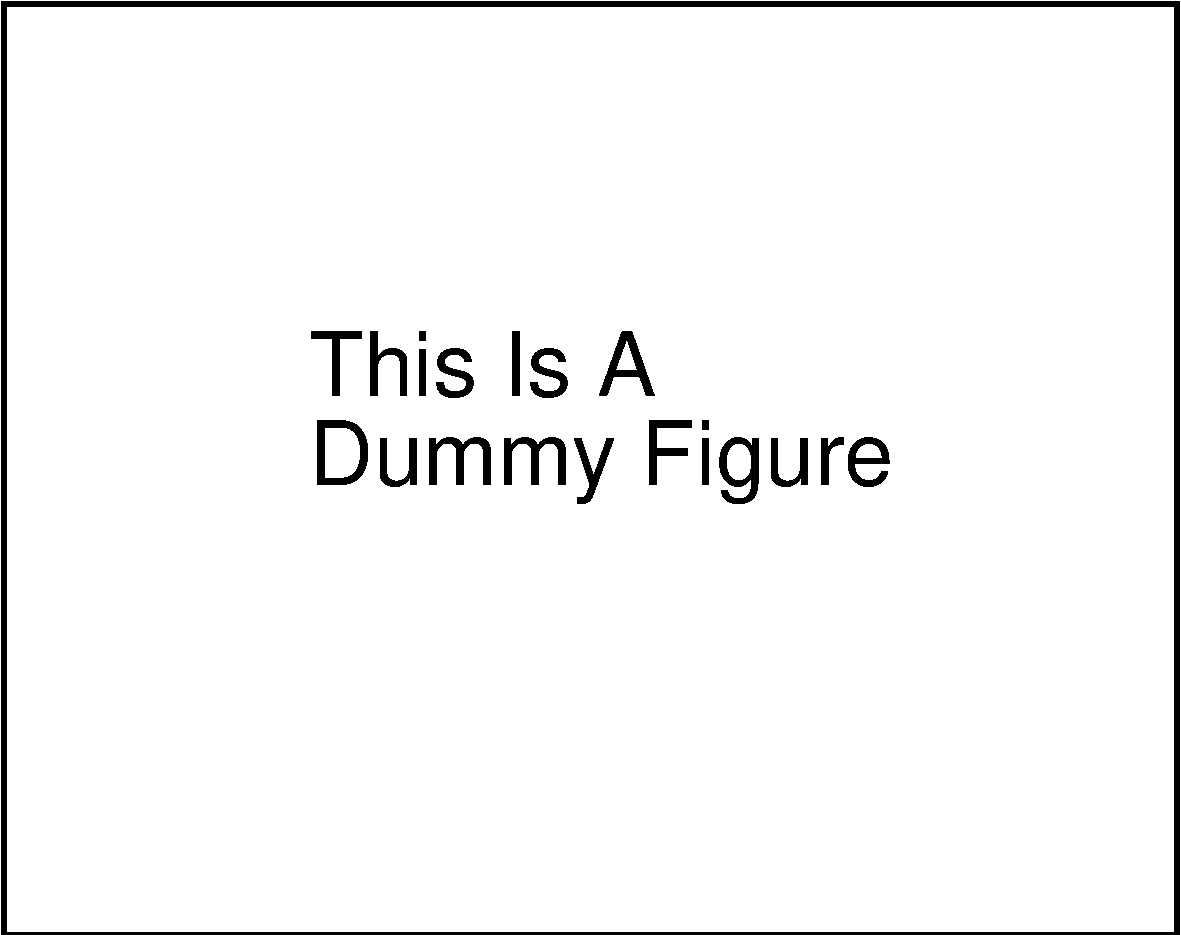
\includegraphics[width=.8\textwidth]{graphics/dummy.pdf}
%\vspace*{6.0cm}
\caption[Expected near detector sensitivity to $\sin^2 \theta_W$ 
for a \MWadj{1.2} beam]{Expected sensitivity to the measurement of $\sin^2 \theta_W$ from the DUNE ND
with the reference \MWadj{1.2} beam and an exposure of $5\times 10^{21}$ POT with a neutrino beam (five years) and 
$5\times 10^{21}$ POT with an antineutrino beam (five years). 
The curve shows the Standard Model prediction as a function of the 
momentum scale~\cite{Czarnecki:2000ic}.
Previous measurements from Atomic Parity Violation~\cite{Bennett:1999zza,Yao:2006px}, Moeller
scattering (E158~\cite{Anthony:2005pm}), $\nu$ DIS (NuTeV~\cite{Zeller:2001hh}) 
and the combined $Z$ pole  measurements (LEP/SLC)~\cite{Yao:2006px}  are also shown for comparison.
The use of a high-energy beam tune
can reduce the DUNE uncertainties by almost a factor of two.
%[figure to be finalized, space holder]
}
\label{fig:sin2thetaw}
\end{figure}
Together, the DIS and the NC elastic scattering channels involve
substantially different scales of momentum transfer, providing a tool
to test the running of $\sin^2 \theta_W$ in a single experiment. To
this end, the study of NC elastic scattering off protons can provide
additional information since it occurs at a momentum scale that is
intermediate between the two other processes.
% Furthermore, in the two NC elastic processes off electrons and
% protons it is possible to reconstruct the $Q^2$, providing
% additional sensitivity.
Figure~\ref{fig:sin2thetaw} summarizes the target sensitivity from the
DUNE ND, compared with existing measurements as a function of the
momentum scale.
In the near future, another precision measurement of $\sin^2 \theta_W$
is expected from the $Q_{\rm weak}$ experiment~\cite{Lee:2013kya}
at Jefferson Laboratory. From the
measurement of parity-violating asymmetry in elastic electron-proton
scattering, the $Q_{\rm weak}$ experiment should achieve a precision
of 0.3\% on $\sin^2 \theta_W$ at $Q^2=0.026$ GeV$^2$.  It should be
noted that the $Q_{\rm weak}$ measurement is complementary to those
from neutrino scattering given the different scale of momentum
transfer and the fact that neutrino measurements are the only direct
probe of the $Z$ coupling to neutrinos. With the \GeVadj{12} upgrade
of Jefferson Laboratory, the $Q_{weak}$ experiment~\cite{Nuruzzaman:2013bwa} could
potentially reach precisions on the order of 0.2-0.1 \%.
%%%%%%%%%%%%%%%%%%%%%%%%%%%%%%%%%%%%%%%%%%%%%%% 
\section{Observation of the Nucleon's Strangeness Content}
\label{sec-deltas} 

  The strange-quark content of the proton and its contribution to the
  proton spin remain enigmatic~\cite{Jaffe:1989jz}.  The question is whether the strange
  quarks contribute substantially to the vector and axial-vector
  currents of the nucleon.  A large observed value of the
  strange-quark contribution to the nucleon spin (axial current),
  $\Delta s$, would enhance our understanding of the proton structure.
The spin structure of the nucleon also affects the couplings of axions and
supersymmetric particles to dark matter. 

\subsection{Strange Form Factors of Nucleons}
The strange quark \emph{vector} elastic form factors\footnote{Nucleon form factors describe the scattering amplitudes off
different partons in a nucleon. They are usually given as a function of
$Q^2$ the momentum transfer to the nucleon from the scattering lepton
(since the structure of the nucleon looks different depending on the
energy of the probe).}
 of the nucleon have been
measured to high precision in parity-violating electron scattering
(PVES) at Jefferson Lab, Mainz and elsewhere.
A recent global analysis~\cite{Young:2006jc} 
of PVES data finds a strange 
magnetic moment $\mu_s = 0.37 \pm 0.79$ (in units of the nucleon
magneton), so that the strange quark contribution to proton magnetic
moment is less than 10\%.
%
For the strange electric charge radius parameter, $\rho_s$, one finds a very
small value, $\rho_s\ = -0.03 \pm 0.63$~GeV$^{-2}$, consistent with zero. 
Both  results are consistent with theoretical expectations
based on lattice QCD and phenomenology~\cite{Leinweber:2004tc}.
In contrast, the strange \emph{axial vector} form factors are poorly 
determined.  A global study of PVES data~\cite{Young:2006jc} 
finds
%
$\widetilde{G}_A^N(Q^2)
= \widetilde{g}_A^N \left( 1 + {Q^2 / M_A^2} \right)^2$,
%
where $M_A = 1.026 $ GeV is the axial dipole mass, with the
effective proton and neutron axial charges 
$\widetilde{g}_A^p = -0.80 \pm 1.68$ and 
$\widetilde{g}_A^n = 1.65 \pm 2.62$.
The strange quark axial form factor at $Q^2=0$ is related to the
\emph{spin} carried by strange quarks, $\Delta s$.
Currently the world data on the spin-dependent $g_1$ structure function
constrain $\Delta s$ to be $\approx -0.055$ at a scale $Q^2=1$~GeV$^2$,
with a significant fraction coming from the region $x < 0.001$. 
An independent extraction of $\Delta s$, which does not rely on the difficult
measurements of the $g_1$ structure function at very small values of the Bjorken variable $x$, can be obtained from (anti)neutrino NC elastic scattering off protons 
 (Figure~\ref{fig-delta-s}). Indeed, 
this process provides the most direct measurement of $\Delta s$.
The differential cross section for NC-elastic and CC-QE scattering of
(anti)neutrinos from protons can be written as:
\begin{equation} \label{eqn:QE}
\frac{d \sigma}{d Q^2} = \frac{G_\mu^2}{2\pi} \frac{Q^2}{E_\nu^2} \left( A \pm BW + C W^2 \right); \;\;\;\;  W=4E_\nu/M_p - Q^2/M_p^2,
\end{equation}
where the positive (negative) sign is for neutrino (antineutrino) scattering and the coefficients
$A, B,$ and $C$ contain the vector and axial form factors as follows:
\begin{eqnarray*}
A & = &  \frac{1}{4} \left[ G_1^2 \left( 1 +\tau \right) - \left( F_1^2 - \tau F_2^2 \right)
\left( 1 - \tau \right) + 4 \tau F_1 F_2 \right]\\
B & = &- \frac{1}{4} G_1 \left( F_1 + F_2 \right)\\
C & = &  \frac{1}{16} \frac{M_p^2}{Q^2} \left( G_1^2 + F_1^2 + \tau F_2^2 \right) \\
\end{eqnarray*}
The axial-vector form factor, $G_1$, for NC scattering can be written as the sum of the known axial
form factor $G_A$ plus a strange form factor $G_A^s$:
\begin{equation}
G_1 = \left[ - \frac{G_A}{2} + \frac{G_A^s}{2} \right],
%\;\;\;\; G_A^s = \frac{\Delta s}{1 + Q^2/M_A^2}
\end{equation}
while the NC vector form factors can be written as:
\begin{equation}
F_{1,2} = \left[ \left(\frac{1}{2} - \sin^2 \theta_W \right) \left( F_{1,2}^p - F_{1,2}^n \right)
- \sin^2 \theta_W \left( F_{1,2}^p + F_{1,2}^n \right) - \frac{1}{2} F_{1,2}^s \right],
\end{equation}
where $F_1^{p(n)}$ is the Dirac form factor of the proton (neutron),
$F_2^{p(n)}$ is the corresponding Pauli form factor, and $F_{1,2}^s$
are the strange-vector form factors.  These latter form factors are
expected to be small from the PVES measurements summarized above.  
In the limit $Q^2 \to 0$, the differential cross section is proportional
to the square of the axial-vector form factor $d \sigma / d Q^2
\propto G_1^2$ and $G_A^s \to \Delta s$.  The value of $\Delta s$ can
therefore be extracted experimentally by extrapolating the NC
differential cross section to $Q^2=0$.
%%%%%%%%%%%%%%%%%%%%%%%%%%%%%  reviewed to here 2/17 11:10 and sent to RP %%%%%%
\subsection{Extraction of the Strange Form Factors}
Previous neutrino scattering experiments have been limited by the
statistics and by the systematic uncertainties on background
subtraction.  One of the earliest measurements available comes from
the analysis of 951 NC $\nu p$ and 776 NC $\overline{\nu}p$ collected
by the experiment BNL
E734~\cite{Ahrens:1986xe,Garvey:1992cg,Alberico:1998qw}. There are
also more recent results with high statistics from MiniBooNE where a
measurement of $\Delta s$ was carried out using neutrino NC elastic
scattering with 94,531 $\nu N$ events~\cite{AguilarArevalo:2010cx}.
The MiniBooNE measurement was limited by the inability to distinguish
the proton and neutron from $\nu N$ scattering. The LBNF neutrino beam
will be sufficiently intense that a measurement of NC elastic
scattering on protons  
in the fine-grained ND can provide a definitive
statement on the contribution of the strange sea to either the axial
or vector form factor.
Systematic uncertainties can be reduced by measuring the NC/CC ratios
for both neutrinos and antineutrinos as a function of $Q^2$:
\begin{equation}
{\cal R}_{\nu p} (Q^2) \equiv \frac{\sigma(\nu_\mu p \to \nu_\mu p)}{\sigma(\nu_\mu n \to \mu^- p)}(Q^2); \;\;\;\;\;
{\cal R}_{\overline{\nu} p} (Q^2) \equiv \frac{\sigma(\overline{\nu}_\mu p \to \overline{\nu}_\mu p)}{\sigma(\overline{\nu}_\mu p \to \mu^+ n)}(Q^2),
\end{equation}
Figure~\ref{fig-delta-s} shows the absolute sensitivity of both ratios
to $\Delta s$ for different values of $Q^2$. The sensitivity for
$Q^2\sim0.25$~GeV$^2$ is about 1.2 for neutrinos and 1.9 for
antineutrinos, which implies that a measurement of ${\cal R}_{\nu p}$
and ${\cal R}_{\overline{\nu} p}$ of 1\% precision would enable the
extraction of $\Delta s$ with an uncertainty of 0.8\% and 0.5\%,
respectively.
%
%---$ Xinchun: "deta-s.pdf"
%
\begin{figure}[!htb]
\centering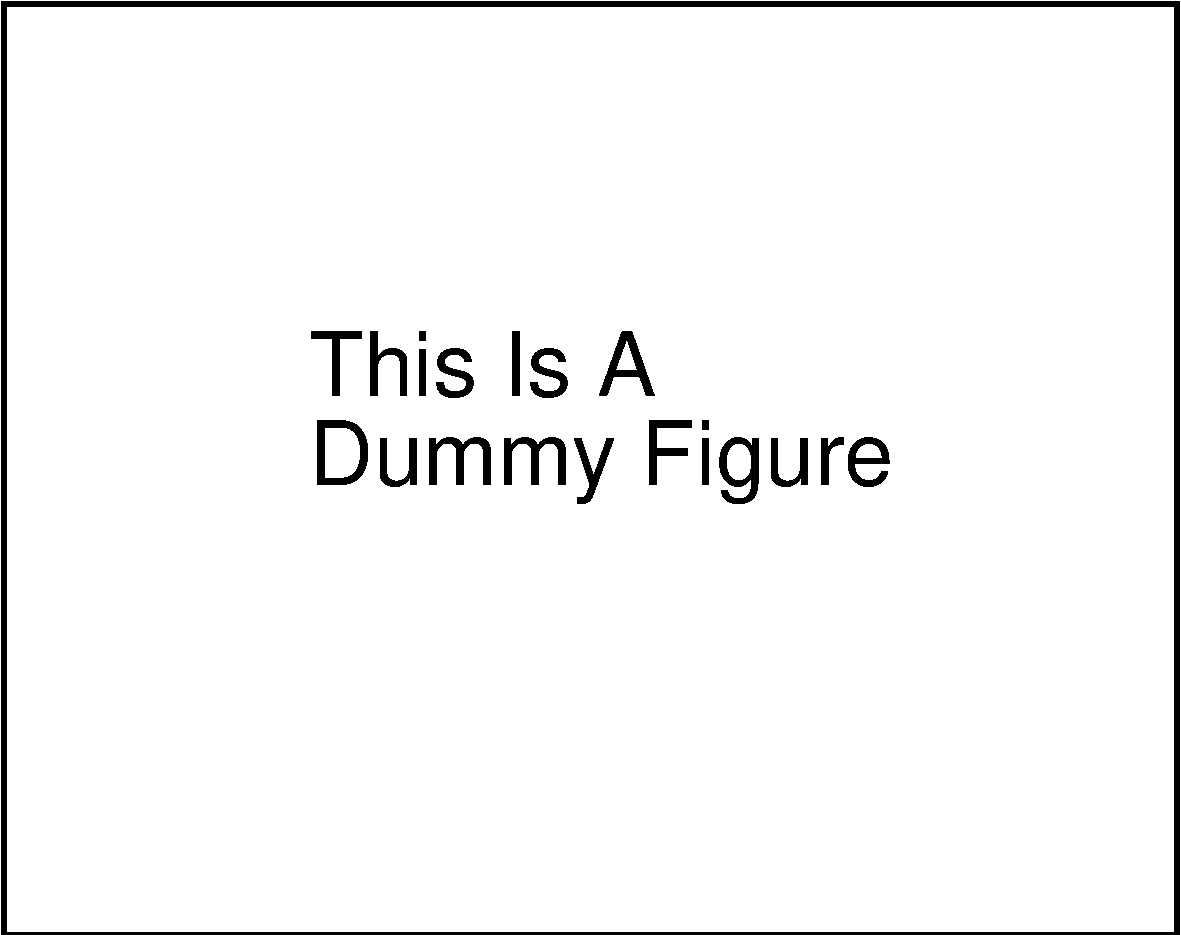
\includegraphics[width=.7\textwidth]{graphics/dummy.pdf}
%\vspace*{6.0cm}
\caption[Sensitivity of NC/CC to the strange contribution to nucleon spin]
{Sensitivity (magnitude) of the ratios ${\cal R}_{\nu p}$ (solid) and
${\cal R}_{\overline{\nu} p}$ (dashed) to a variation of the strange contribution to the
spin of the nucleon, $\Delta s$,
as a function of $Q^2$. Values greater than one imply that the relative uncertainty on $\Delta s$ is smaller than that of the corresponding ratio (see text).}
\label{fig-delta-s}
\end{figure}
The design of the %high-resolution tracker ND 
tracker includes several
different nuclear targets.  Therefore, most of the neutrino scattering
is from nucleons embedded in a nucleus, requiring nuclear effects to
be taken into account. Fortunately, in the ratio of NC/CC, the nuclear
corrections are expected to largely cancel out.  The $\Delta s$
analysis requires a good proton reconstruction efficiency as well as
high resolution on both the proton angle and energy. To this end, the
low-density %magnetized tracker at DUNE 
tracker can increase the range of the
protons inside the ND, allowing the reconstruction of proton tracks
down to $Q^2\sim0.07$~GeV$^2$. This capability will reduce the
uncertainties in the extrapolation of the form factors to the limit
$Q^2 \to 0$.
Table~\ref{tab:prange} summarizes the expected proton range for the
low-density ($\rho\sim$~\SI{0.1}{\gram\per\cubic\centi\meter}) straw-tube 
tracker (STT) in the ND tracking detector design described in
Section~\ref{sec:ndproj}.  About $2.0 (1.2) \times 10^6$ $\nu p
(\overline{\nu} p)$ events are expected after the selection cuts in
the low-density 
tracker, yielding a statistical precision on the order
of 0.1\%.
\begin{table}[htb]
\centering
\caption[Expected proton range for the  low-density tracker]{Expected proton range for the  low-density
($\rho\sim$\SI{0.1}{\gram\per\cubic\centi\meter}) tracker. The first column gives the proton kinetic energy
and the last column the proton momentum. The $Q^2$ value producing $T_p$ is calculated
assuming the struck nucleon is initially at rest.}
\label{tab:prange}
\begin{tabular}{$L^c^r^c}  %{$l^l^l^l^l^l}
\toprule
\rowtitlestyle
$ T_p$  &  $Q^2$          &  Range STT &  $P_p$  \\
\rowtitlestyle
MeV  &  GeV$^2/c^2$ &  $cm$        &  GeV$/c$ \\ 
\toprowrule
         20 &             0.038  &     4.2          & 0.195  \\ \colhline
        40 &              0.075  &   14.5          & 0.277  \\ \colhline
        60 &              0.113  &   30.3          & 0.341   \\ \colhline
        80 &              0.150  &  50.8          & 0.395  \\ \colhline
      100 &               0.188 &  75.7          & 0.445  \\ 
\bottomrule
\end{tabular}
\end{table}
The determination of $\Delta s$ in the STT %straw-tube tracker ND 
utilizes
analysis techniques performed by the FINeSSE
Collaboration~\cite{Bugel:2004yk} and used by the SciBooNE experiment.  In
particular, based on the latter, DUNE
expects a purity of about 50\%, with background contributions of 20\%
from neutrons produced outside of the detector, 10\% $\nu n$ events
and 10\% NC pion backgrounds.  The dominant systematic uncertainty
will be related to the background subtraction.  The low-energy beam
spectrum at DUNE provides the best sensitivity for this measurement
since the external background from neutron-induced proton recoils will
be reduced by the strongly suppressed high-energy tail.  The
low-density magnetized tracker is expected to increase the purity by
reducing the neutron background and the NC pion background.  The
outside neutron background, it should be noted, can be determined
using the $n \rightarrow p + \pi^-$ process in the STT.  The
sensitivity analysis is still in progress, however DUNE is confident
of achieving a precision on $\Delta s$ of about \numrange[range-phrase
= --]{0.02}{0.03}.
 
\clearpage
%%%%%%%%%%%%%%%%%%%%%%%%%%%%%%%%%%%%%%%%%%%%%%%
\section{Nucleon Structure and QCD Studies}
\label{sec-nucleon}

  Precision measurements of (anti)neutrino differential cross sections
  in the DUNE near detector will provide additional constraints on
  several key nucleon structure functions that are complementary to
  results from electron scattering experiments.
  In addition, these measurements would directly improve DUNE's
  oscillation measurements by providing accurate simulation of
  neutrino interactions in the far detector and offer an estimate of
  all background processes that are dependent upon the angular
  distribution of the outgoing particles in the far detector.
%
  Furthermore, certain QCD analyses --- i.e., global fits used for extraction of
  parton distribution functions (PDFs) via 
  the differential cross sections measured in ND data ---
  would constrain the systematic error in 
  precision electroweak measurements. This would apply  
  not only in neutrino physics but also in hadron collider measurements.  

%%%%%%%%%%%%%%%%%%%%%%%%%
\subsection{\boldmath Determination of the $F_3$
Structure Function and GLS Sum Rule}
For quantitative studies of inclusive deep-inelastic lepton-nucleon
scattering, it is vital to have precise measurements of the $F_3$
structure functions as input into global PDF fits.  Because it depends
on weak axial quark charges, the $F_3$ structure function can only be
measured with neutrino and antineutrino beams and is unique in its
ability to differentiate between the quark and antiquark content of
the nucleon.  On a proton target, for instance, the neutrino and
antineutrino $F_3$ structure functions (at leading order in
$\alpha_s$) are given by
%
\begin{eqnarray}
xF_3^{\nu p}(x) 
&=& 2 x \left( d(x) - \overline u(x) + s(x) + \cdots \right)\, , \\
%
xF_3^{\overline\nu p}(x) 
&=& 2 x \left( u(x) - \overline d(x) - \overline s(x) + \cdots \right)\, , \\ 
xF_3^{\nu n}(x) 
&=& 2 x \left( u(x) - \overline d(x) + s(x) + \cdots \right)\, , \\
%
xF_3^{\overline\nu n}(x) 
&=& 2 x \left( d(x) - \overline u(x) - \overline s(x) + \cdots \right)\, .
\end{eqnarray}
where $u_v=u-\bar u$ and $d_v=d-\bar d$ are the valence sea quark
distributions. Under the assumption of a symmetric strange sea,
i.e., $s(x)=\bar s(x)$, the above expressions show that a measurement
of the average $xF_3=(xF_3^{\nu N}+xF_3^{\bar\nu N})/2$ for neutrino
and antineutrino interactions on isoscalar targets provides a direct
determination of the valence quark distributions in the proton. This
measurement is complementary to the measurement of Drell-Yan
production at colliders, which is essentially proportional to the sea
quark distributions.
\clearpage
The first step in the structure function analysis is the measurement
of the differential cross section:
\begin{equation} 
\frac{1}{E_\nu} \frac{d \sigma^2}{dx dQ^2} = \frac{N(x,Q^2,E_\nu)}{N(E_\nu)} \frac{\sigma_{\rm tot}/E_\nu}{dx dQ^2} 
\end{equation} 
where $N(x,Q^2,E_\nu)$ is the number of events in each $(x,Q^2,E_\nu)$ bin and $N(E_\nu)$ is the number of events in each $E_\nu$ 
bin integrated over $x$ and $Q^2$. The average $xF_3$ structure function can be extracted by taking the difference between neutrino and 
antineutrino differential cross sections: 
\begin{equation} 
\frac{1}{E_\nu} \frac{d^2 \sigma^\nu}{dx dQ^2} - \frac{1}{E_\nu} \frac{d^2 \sigma^{\bar \nu}}{dx dQ^2} = 2 \left[ y \left( 1 - \frac{y}{2} \right) \frac{y}{Q^2} \right] xF_3  
\end{equation} where $xF_3$ denotes the sum for neutrino and antineutrino interactions. 
The determination of the $xF_3$ structure functions will, in turn,
allow a precision measurement of the Gross-Llewellyn-Smith (GLS) QCD
sum rule:
\begin{eqnarray}
\label{eq:GLS}
S_{\rm GLS} (Q^2) & = & 
\frac{1}{2} \int^1_0 \frac{1}{x} \left[ xF_3^{\nu N} + xF_3^{\bar \nu N} \right] dx \nonumber \\ 
& = & 3 \left[ 1 - \frac{\alpha_s(Q^2)}{\pi} - a(n_f) \left( \frac{\alpha_s(Q^2)}{\pi} \right)^2
-b(n_f) \left( \frac{\alpha_s(Q^2)}{\pi} \right)^3 \right] + \Delta {\rm HT}
\end{eqnarray}
where $\alpha_s$ is the strong coupling constant, $n_f$ is the number
of quark flavors, $a$ and $b$ are known functions of $n_f$, and the
quantity $\Delta {\rm HT}$ represents higher-twist contributions.  The
equation above can be inverted to determine $\alpha_s(Q^2)$ from the
GLS sum rule. The most precise determination of the GLS sum rule was
obtained by the CCFR experiment on an iron target~\cite{Leung:1992yx}
$S_{\rm GLS} (Q^2=3~GeV^2) = 2.50 \pm 0.018 \pm 0.078$. %The use of a
The high-resolution ND combined with the unprecedented statistics
would substantially reduce the systematic uncertainty on the low-$x$
extrapolation of the $xF_3$ structure functions entering the GLS
integral.  In addition, the presence of different nuclear targets, as
well as the availability of a target with free protons
will allow investigation of isovector and nuclear corrections, and
adding a tool to test isospin (charge) symmetry (Section~\ref{sec-isospin}).
%%%%%%%%%%%%%%%%%%%%%%%%%
\subsection{\boldmath Determination of the Longitudinal Structure Function $F_L(x,Q^2)$}
The structure
function $F_L$ is directly related to the gluon distribution
$G(x,Q^2)$ of the nucleon, as can be seen from the
Altarelli-Martinelli relation:
\begin{equation} 
F_L(x,Q^2) = \frac{\alpha_s(Q^2)}{\pi} \left[ \frac{4}{3}\int^1_x \frac{dy}{y} \left(\frac{x}{y} \right)^2 F_2(x,Q^2) + 
n_f \int^1_x \frac{dy}{y}\left(\frac{x}{y} \right)^2 \left( 1-\frac{x}{y} \right) G(y,Q^2) \right]
%2\sum_i e_i^2 \int^1_x \frac{dy}{y}\left(\frac{x}{y} \right)^2 \left( 1-\frac{x}{y} \right) G(y,Q^2) \right]  
\end{equation}  
where $n_f$ is the number of parton flavors. In the leading order 
approximation the longitudinal structure function $F_L$ is zero, while
at higher orders a nonzero $F_L(x,Q^2)$ is originated as a consequence of the violation
of the Callan-Gross relation:
\begin{equation} 
F_L(x,Q^2) = \left(  1+\frac{4M^2x^2}{Q^2} \right) F_2(x,Q^2) - 2x F_1(x,Q^2) 
\end{equation}  
where $2x F_1=F_T$ is the transverse structure function.  A
measurement of $R=F_L/F_T$ is therefore both a test of perturbative QCD at
large $x$ and a clean probe of the gluon density at small $x$ where the
quark contribution is small. A poor knowledge of $R$, especially at
small $x$, results in uncertainties in the structure functions extracted
from deep inelastic scattering cross sections, and in turn, in
electroweak measurements.  It is instructive to compare the low-$Q^2$
behavior of $R$ for charged-lepton versus  neutrino scattering. In both
cases CVC implies that $F_T \propto Q^2$ as $Q^2 \to 0$. However,
while $F_L \propto Q^4$ for the electromagnetic current, for the weak
current $F_L$ is dominated by the finite PCAC (partial conservation of
the axial current) contribution \cite{Kulagin:2007ju}.
The behavior of
$R$ at $Q^2\ll 1$ GeV$^2$ is therefore very different for
charged-lepton and neutrino scattering.  A new precision measurement
of the $Q^2$ dependence of $R$ with (anti)neutrino data would also
clarify the size of the high-twist contributions to $F_L$ and $R$,
which reflect the strength of multi-parton correlations (qq and
qg). 
The ratio of longitudinal to transverse structure functions can be
measured from the $y$ dependence of the deep inelastic scattering
data. Fits to the following function:
\begin{equation} 
F(x,Q^2, \epsilon) = \frac{\pi (1- \epsilon)}{y^2 G_F^2 M E_\nu} \left[ \frac{d^2 \sigma^\nu}{dx dy} + \frac{d^2 \sigma^{\bar \nu}}{dx dy} \right] = 2 x F_1(x,Q^2) \left[ 1 + \epsilon R(x,Q^2) \right] 
\end{equation} 
have been used by CCFR and NuTeV to determine
$R=\sigma_L/\sigma_T$. In this equation $\epsilon \simeq 2
(1-y)/(1+(1-y)^2)$ is the polarization of the virtual $W$ boson. This
equation assumes $xF_3^\nu = xF_3^{\bar \nu}$, and a correction must be
applied if this is not the case. The values of $R$ are extracted from
linear fits to $F$ versus $\epsilon$ at fixed $x$ and $Q^2$ bins.
%%%%%%%%%%%%%%%%%%%%%%%%%
\subsection{\boldmath Determination of $F_2^n$ and the $d/u$ Ratio of Quark Distribution Functions}
Because of the larger electric charge on the $u$ quark than on the
$d$, the electromagnetic proton $F_2$ structure function data provide
strong constraints on the $u$-quark distribution, but are relatively
insensitive to the $d$-quark distribution.  To constrain the $d$-quark
distribution a precise knowledge of the corresponding $F_2^n$
structure functions of free neutrons is required, which in current practice is
%currently 
extracted from inclusive deuterium $F_2$ data.  At large values of $x$
($x>0.5$) the nuclear corrections in deuterium become large and, more
importantly, strongly model-dependent, leading to large uncertainties
on the resulting $d$-quark distribution.  Using the isospin relation
$F_2^{\bar \nu p} = F_2^{\nu n}$ and $F_2^{\nu p} = F_2^{\bar \nu n}$
it is possible to obtain a direct determination of $F_2^{\nu n}$ and
$F_2^{\bar \nu n}$ with neutrino and antineutrino scattering off a target with free
protons. This determination is free from model uncertainties
related to nuclear targets. The extraction of $F_2^{\nu n}$ and
$F_2^{\bar \nu n}$ will allow a precise extraction on the $d$-quark
distribution at large $x$.  Existing neutrino data on hydrogen  
have relatively large errors and do not extend beyond
$x\sim0.5$~\cite{Bodek:1985tv,Jones:1987gk}.
The $F_2^{\bar \nu p}$ and $F_2^{\nu p}$ structure functions can be
obtained from interactions on a target with free protons  after subtracting
the contributions from $xF_3$ and $R$. These latter can either be
modeled within global PDF fits or taken from the other two
measurements described above. As discussed in Section~\ref{sec-isospin} the DUNE 
ND can achieve competitive measurements of $F_2^{\bar \nu p}$ and $F_2^{\nu p}$ 
with an increase of statistics of three orders of magnitude with respect to the 
existing hydrogen data~\cite{Bodek:1985tv,Jones:1987gk}. 
%%%%%%%%%%%%%%%%%%%%%%%%%
\subsection{Measurement of Nucleon Structure Functions}
At present neutrino scattering measurements of cross sections have
considerably larger uncertainties than those of the electromagnetic
inclusive cross sections.  The measurement of the differential cross
sections~\cite{Formaggio:2013kya} is dominated by three
uncertainties: (1) muon energy scale, (2) hadron energy scale, and (3)
knowledge of the input (anti)neutrino flux.  Table~\ref{tab:expcomp}
shows a comparison of past and present experiments and the
corresponding uncertainties on the energy scales.  The most precise
measurements are from the CCFR, NuTeV and NOMAD experiments, which are
limited to a statistics of about \num{e6} neutrino events.
%
\begin{dunetable}[Structure function measurements from previous experiments]{lccccrr}{expcomp}
  {Summary of past experiments performing structure function measurements. The expected numbers in the DUNE near detector for a five-year run with the \SIadj{1.2}{\MW} \SIadj{120}{\GeV} reference beam  ($5 \times 10^{21}$ POT) are also given for comparison.}  
Experiment & Mass & \multicolumn{1}{c}{\numu CC Stat.} & Target & $E_\nu$ (GeV)
& $\Delta E_\mu$  & $\Delta E_{\rm H}$ \\ \toprowrule
            CDHS~\cite{Berge:1989hr} &  750 t &  { $10^{7}$}   &  p,Fe & 20-200 & 2.0\% & 2.5\% \\ \colhline
%    CHARM II  &  547 t  & { $10^{7}$}  & SiO$_2$ & 20-200 & & \\
            BEBC~\cite{Allasia:1983vw,Allasia:1985hw} & various &   5.7$\times$$10^{4}$   & p,D,Ne & 10-200 &  & \\ \colhline
            CCFR~\cite{Yang:2000ju,Yang:2001xc} & 690 t & { 1.0$\times$$10^{6}$}   & Fe & 30-360 & 1.0\% & 1.0\% \\  \colhline
            NuTeV~\cite{Tzanov:2005kr} &  690 t & { 1.3$\times$$10^{6}$}  &  Fe &  30-360 &  0.7\% &  0.43\% \\ \colhline
            CHORUS~\cite{Onengut:2005kv} & 100 t & { 3.6$\times$$10^{6}$}   &  Pb &  10-200 &  2.5\% &  5.0\% \\ \colhline
            NOMAD~\cite{Wu:2007ab} & 2.7 t & { 1.3$\times$$10^{6}$}   &  C &  5-200 &  0.2\% &  0.5\% \\ \colhline
            ~~~~~~~~~~~~~~~~~\cite{Samoylov:2013xoa}     & 18 t & { 1.2$\times$$10^{7}$}   &  Fe  &  5-200 &  0.2\% &  0.6\% \\ \colhline
            MINOS ND~\cite{Adamson:2009ju} & 980 t &  3.6$\times$$10^{6}$   &  Fe & 3-50 & 2-4\% & 5.6\% \\  \colhline
            DUNE ND  & 5 t &  5.9$\times$$10^{7}$   & (C$_3$H$_6$)$_n$  & 0.5-30 & $<0.2$\% & $<0.5$\% \\  \bottomrule
\end{dunetable} 

The MINER$\nu$A~\cite{Osmanov:2011ig} experiment is expected to provide new structure
function measurements on a number of nuclear targets including He, C,
Fe and Pb in the near future.  Since the structure function
measurement mainly involves DIS events, the MINER$\nu$A measurement
will achieve a competitive statistics after the completion of the new
run with the medium-energy beam. 
MINER$\nu$A will focus on a measurement of the ratio of different nuclear
targets to measure nuclear corrections in (anti)neutrino
interactions. It must be noted that the MINER$\nu$A experiment relies
on the MINOS ND for muon identification.  The corresponding
uncertainty on the muon-energy scale (Table~\ref{tab:expcomp}) is
substantially larger than that in other modern experiments, e.g.,
NuTeV and NOMAD, thus limiting %. This fact would limit 
the potential of absolute
structure function measurements. Furthermore, the muon-energy scale is
also the dominant source of uncertainty in the determination of the
(anti)neutrino fluxes with the low-$\nu$ method.  Therefore, the flux
uncertainties in MINER$\nu$A are %also 
expected to be larger than in
NOMAD and NuTeV. 
 
Given its reference beam design and \MWadj{1.2} proton-beam power, DUNE
expects to collect about \num{2.3e7} neutrino DIS events and
about \num{4.4e6}  antineutrino DIS events in the ND. 
These numbers correspond to an improvement
by more than one order of magnitude with respect to the most precise
past experiments, e.g., NuTeV~\cite{Tzanov:2005kr} and 
NOMAD~\cite{Wu:2007ab,Samoylov:2013xoa}. 
With these high-statistics
samples, DUNE will be able to significantly reduce the gap between the
uncertainties on the weak and electromagnetic structure functions.
A possible high-energy run with the upgraded \MWadj{2.3} beam would offer a 
further increase by more than a factor of ten in statistics.  
In addition to the large data samples, the use of a high-resolution,
low-density spectrometer allows DUNE to reduce systematic
uncertainties with respect to previous measurements. The DUNE ND is
expected to achieve precisions better than 0.2\% and 0.5\% on the muon-
and hadron-energy scales, respectively. 
These numbers are based on the results achieved by the NOMAD experiment
(Table~\ref{tab:expcomp}), which had %a much smaller statistics 
much lower statistics and
poorer resolution than is expected in the DUNE ND. The calibration of the momentum and energy scales
will be performed with the large sample of reconstructed $K^0_S \to \pi \pi$,
$\Lambda \to p \pi$, and $\pi^0 \to \gamma \gamma$ decays.
In addition, the overall hadronic energy scale can be calibrated by exploiting the
well-known structure of the Bjorken $y$ distribution in (anti)neutrino DIS
interactions~\cite{Wu:2007ab,Petti:2011zz}.
%  
The relative fluxes as a function of energy can be extracted to a precision of 
about 2\% with the low-$\nu$ method, due to the small uncertainty on the muon-energy
scale. The world average absolute normalization of the differential
cross sections $\sigma_{\rm tot}/E$, is known to 2.1\%
precision~\cite{Beringer:1900zz}. 
However, with the \MWadj{1.2} beam available from the PIP-II
upgrades, it will be possible to improve the absolute normalization
using $\nu$-e NC elastic scattering events, coherent meson production, etc. 
An overall precision of 1-2\% would make (anti)neutrino
measurements comparable to or better than the complementary measurements from
charged-lepton DIS.
On the time scale of %the DUNE project
DUNE, comparable measurements from
(anti)neutrino experiments are not expected, primarily due to the low
energy of competing beamlines (J-PARC neutrino beamline in Japan~\cite{Sekiguchi:2012xma}) or to the poorer resolution of the detectors
used (MINER$\nu$A~\cite{Osmanov:2011ig} , T2K~\cite{Abe:2011ks},
NO$\nu$A~\cite{Ayres:2007tu}). The %main 
experimental program %that can
most likely to compete with the DUNE ND measurements is the \GeVadj{12} upgrade at
Jefferson Laboratory (JLab)~\cite{Dudek:2012vr}.  However, it must be
emphasized that the use of electron beams at JLab makes this program
\emph{complementary} to DUNE's.  In particular, the three topics
discussed above are specific to the (anti)neutrino interactions.
Several planned experiments at JLab with the energy-upgraded \GeVadj{12}
beam will measure the $d/u$ ratio from D targets up to $x\sim0.85$, 
using different methods to minimize the nuclear corrections.  
The DUNE measurement %in the ND 
will be competitive with the
proposed JLab \GeVadj{12} experiments, since the large statistics expected will allow
a precise determination of $F_2^{\nu
  n}$ and $F_2^{\bar \nu n}$ up to $x\sim0.85$. Furthermore,
the use of a weak probe coupled with a wide-band beam will provide
a broader $Q^2$ range than in JLab experiments, thus allowing a separation of
higher twist and other sub-leading effects in $1/Q^2$.
%%%%%%%%%%%%%%%%%%%%%%%%%%%%%%%%%%%%%%%%%%%%%%%
\section{Tests of Isospin Physics and Sum-Rules}
%\section{Isospin Physics and Sum-Rules}
\label{sec-isospin}

One of the most compelling physics topics accessible to DUNE's high-resolution near detector is the isospin physics using neutrino and antineutrino interactions. This physics involves the Adler sum rule and tests isospin (charge) symmetry in nucleons and nuclei.

The Adler sum rule relates the integrated difference of the
antineutrino and neutrino $F_2$ structure functions to the isospin of the target:
%
\begin{equation}
\label{ASR}
{\cal S}_A (Q^2) =\int_0^1 \; dx \; \left[ F_2^{\overline\nu} (x,Q^2) - F_2^{\nu}(x,Q^2) \right]/(2x)
= 2\,I_z,
\end{equation}
%
where the integration is performed over the entire kinematic range of the
Bjorken variable $x$ and $I_z$ is the projection of
the target isospin vector on the quantization axis ($z$ axis).
For the proton ${\cal S}_A^{p}=1$ and for the neutron ${\cal S}_A^{n}=-1$.
In the quark-parton model the Adler sum is the difference between the
number of valence $u$ and $d$ quarks of the target. The Adler sum rule
survives the strong-interaction effects because of the conserved vector 
current (CVC) and provides an
exact relation to test the local current commutator algebra of the weak
hadronic current. %We note that 
In the derivation of the Adler sum rule the effects of both
non-conservation of the axial current and heavy-quark production are
neglected. 
Experimental tests of the Adler sum rule require the use of a hydrogen target
to avoid nuclear corrections to the bound nucleons inside the nuclei.
The structure functions $F_2^{\overline{\nu}}$ and $F_2^\nu$ have to be determined
from the corresponding differential cross sections and must be extrapolated
to small $x$ values in order to evaluate the integral. %~(\ref{ASR}). 
The test performed in bubble chambers by the BEBC
Collaboration --- the only test available ---  is limited by the modest statistics;
it used about 9,000 $\overline{\nu}$ and 5,000 $\nu$ events
collected on hydrogen~\cite{Allasia:1985hw}.
The DUNE program can provide the first high-precision test of the
Adler sum rule.  To this end, the use of the high-energy beam tune
shown in Figure~\ref{fig:beamtunes}, although not essential, would
increase the sensitivity, allowing attainment of higher $Q^2$
values. Since the use of a liquid H$_2$ bubble chamber is excluded in
the ND hall due to safety concerns, the (anti)neutrino interactions
off a hydrogen target can only be extracted with a subtraction method
from the composite materials of the ND targets.  Using this technique
to determine the position resolution in the location of the primary
vertex is crucial to reducing systematic uncertainties.  For this
reason, a precision test of the Adler sum rule is best performed with
the low-density magnetized ND.
A combination of two different targets --- the polypropylene
$(C_3H_6)_n$ foils placed in front of the STT modules and pure carbon
foils --- are used in the low-density, magnetized 
ND to provide a
fiducial hydrogen mass of about 1 t.  With the DUNE fluxes from
the standard exposure, $5.0(1.5) \times 10^6 \pm 13(6.6)\times 10^3
(sub.)$ $\nu(\overline{\nu})$ CC events (where the quoted uncertainty is dominated by the
statistical subtraction procedure) %about \num{1e6} inclusive
%$\nu(\overline{\nu})$ CC events 
would be collected on the hydrogen
target.  The level of precision that can be achieved is sufficient to
open up the possibility of making new discoveries in the quark and
hadron structure of the proton. No other comparable measurement is
expected on the timescale of DUNE.
%%%%%%%%%%%%%%%%%%%%%%%%%%%%%%%%%%%%%%%%%%%%%%%
\section{Studies of (Anti)Neutrino-Nucleus Interactions} 
\label{sec-nuclear} 
An integral part of the physics program envisioned for the DUNE ND
involves detailed measurements of (anti)neutrino interactions in a
variety of nuclear targets.  The DUNE ND offers substantially
larger statistics coupled with a much higher resolution and, in turn,
lower systematic uncertainties with respect to past experiments
(Table~\ref{tab:expcomp}) or ongoing and future ones
(MINER$\nu$A~\cite{Osmanov:2011ig}, T2K~\cite{Abe:2011ks},
NO$\nu$A~\cite{Ayres:2007tu}).  The most important nuclear target is
of course the argon target, which matches the DUNE far detector.
%Regarding 
The ND standard target is polypropylene
(C$_3$H$_6$)$_n$, largely provided by the mass of the STT radiators.
%
An additional proposed ND target is argon gas in pressurized aluminum
tubes with sufficient mass to provide $\simeq$10 times the \numu CC and
NC statistics as expected in the DUNE far detector.  Equally important
nuclear targets are carbon (graphite), which is essential in order to
get (anti)neutrino interactions on free protons through a statistical
subtraction procedure from the main polypropylene target 
(Section~\ref{sec-isospin}), and calcium.  In particular, this latter
target has the same atomic weight ($A=40$) as argon but is
isoscalar. One additional nuclear target is iron, which is used in the
proposed India-based Neutrino Observatory
(INO)~\cite{Mondal:2012fn}. %Indeed t
The modularity of the STT provides for successive measurements using
thin nuclear targets (thickness $< 0.1 X_0$), while the excellent
angular and space resolution allows a clean separation of events
originating in different target materials.  Placing an arrangement of
different nuclear targets upstream of the detector
provides the desired nuclear samples in (anti)neutrino interactions.
For example, a single \SIadj{7}{\milli\meter}-thick calcium layer at the upstream 
end of the detector will provide  
about \num{3.1e5} \numu CC interactions in one year. 
%
Potential ND studies in nuclear effects include the following: 
%
\begin{itemize}%[parsep=-2pt]
\item nuclear modifications of form factors
\item nuclear modifications of structure functions
\item mechanisms for nuclear effects in coherent and incoherent regimes
\item a dependence of exclusive and semi-exclusive processes
\item effect of final-state interactions
\item effect of short-range correlations
\item two-body currents
\end{itemize}
The study of nuclear effects in (anti)neutrino interactions off nuclei
is directly relevant for the long-baseline oscillation studies.  The
use of heavy nuclei like argon in the DUNE far detector requires a measurement
of nuclear cross sections on the same targets in the ND in order to reduce signal 
and background uncertainties in the oscillation analyses.  Cross-section
measurements obtained from other experiments using different nuclei
are not optimal; in addition to the different $p/n$ ratio in argon
compared to iron or carbon where measurements from other experiments
exist, nuclear modifications of cross sections can differ from 5\% to
15\% between carbon and argon for example, while the difference in the
final-state interactions could be larger.
%~\cite{docdb740}.
Additionally, nuclear modifications can introduce a substantial
smearing of the kinematic variables reconstructed from the observed
final-state particles.  Detailed measurements of the dependence on the
atomic number $A$ of different exclusive processes are then required
in order to understand the absolute energy scale of neutrino event
interactions and to reduce the corresponding systematic uncertainties
on the oscillation parameters.
It is worth noting that the availability of a free-proton target
through statistical subtraction of the (C$_3$H$_6$)$_n$ and carbon
targets (Section~\ref{sec-isospin}) will allow for the first time a
direct model-independent measurement of nuclear effects --- including
both the primary and final-state interactions --- on the argon target
relevant for the far detector oscillation analysis.
Furthermore, an important question in nuclear physics is how the
structure of a nucleon is modified when said nucleon is inside the
medium of a heavy nucleus as compared to a free nucleon like the
proton in a hydrogen nucleus.  Studies of the ratio of structure
functions of nuclei to those of free nucleons (or in practice, the
deuteron) reveal nontrivial deviations from unity as a function of $x$
and $Q^2$.  These have been well explored in charged-lepton scattering
experiments, but little empirical information exists from neutrino
scattering. Measurements of structure using neutrino scattering are
complementary to those in charged-lepton scattering.
Another reason to investigate the nuclear-medium modifications 
of neutrino structure functions is that most neutrino scattering
experiments are performed on nuclear targets, from which information
on the free nucleon is inferred by performing a correction for the
nuclear effects.  
%
In practice this often means applying the same nuclear correction as
for the electromagnetic structure functions, which introduces an
inherent model-dependence in the result.  In particular, significant
differences between photon-induced and weak-boson-induced nuclear
structure functions are predicted, especially at low $Q^2$ and low
$x$, which have not been tested.  A striking example is offered by the
ratio $R$ of the longitudinal-to-transverse structure
functions~\cite{Kulagin:2007ju}.  While the electromagnetic ratio tends
to zero in the photoproduction limit, $Q^2 \to 0$, by current
conservation, the ratio for neutrino structure functions is predicted
to be \emph{finite} in this limit.  Thus, significant discovery
potential exists in the study of neutrino scattering from nuclei.
The comparison of argon and calcium targets (${}^{40}_{18}$Ar and
${}^{40}_{20}$Ca) in the DUNE ND would be particularly
interesting. Since most nuclear effects depend on the atomic weight
$A$, inclusive properties of (anti)neutrino interactions are expected
to be the same for these two
targets~\cite{Kulagin:2007ju,Butkevich:2012zr,Butkevich:2007gm,Ankowski:2007uy}.
This fact would allow the use of both targets to model signal and
backgrounds in the DUNE far detector (argon target), as well as to
compare DUNE results for nuclear effects on argon with the extensive
data on calcium from charged lepton DIS. In addition, a high-precision
measurement of (anti)neutrino interactions in both argon and calcium
opens the possibility for studying a potential flavor and isovector
dependence of nuclear effects and to further test the isospin (charge
symmetry) in nuclei (Section~\ref{sec-isospin}).  Evidence for any
of these effects would constitute important discoveries.
Finally, the extraction of (anti)neutrino interactions on deuterium
from the statistical subtraction of H$_2$O from D$_2$O, which is
required to measure the fluxes (Section~\ref{sec-fluxosc}), would
allow the first direct measurement of nuclear effects in deuterium.
This measurement can be achieved since the structure function of a
free isoscalar nucleon is given by the average of neutrino and
antineutrino structure functions on hydrogen ($F_2^{\nu
  n}=F_2^{\overline{\nu} p}$).  A precise determination of nuclear
modifications of structure functions in deuterium would play a crucial
role in reducing systematic uncertainties from the global PDF fits.
%%%%%%%%%%%%%%%%%%%%%%%%%%%%%%%%%%%%%%%%%%%%%%%
\section{Search for Heavy Neutrinos} 

  The most economical way to handle the problems of neutrino masses,
  dark matter and the Baryon Asymmetry of the Universe in a unified
  way may be to add to the Standard Model (SM) three Majorana singlet
  fermions with masses roughly on the order of the masses of known
  quarks and leptons using the seesaw
  mechanism~\cite{Yanagida:1980xy}. The appealing feature of this
  theory (called the $\nu$MSM for \emph{Neutrino Minimal
    SM})~\cite{Asaka:2005pn} is that every left-handed fermion has a
  right-handed counterpart, leading to a consistent way of treating
  quarks and leptons.
  The most efficient mechanism proposed for producing these heavy
  sterile singlet states experimentally is through weak decays of
  heavy mesons and baryons, as can be seen from the left-hand diagram
  in Figure~\ref{fig:production-and-decays}, showing some examples of
  relevant two- and three-body decays~\cite{Gorbunov:2007ak}. These
  heavy mesons can be produced by energetic protons scattering off the
  DUNE neutrino production target and the heavy singlet neutrinos from their
  decays detected in the near detector.

\begin{figure}[!htb]
\centering
\tikzset{
  quark/.style={draw=blue, postaction={decorate},
    decoration={markings,mark=at position .6 with {\arrow[draw=blue]{>}}}},
  electron/.style={draw=pink, postaction={decorate},
    decoration={markings,mark=at position .6 with {\arrow[draw=blue]{>}}}},
  neutrino/.style={draw=red, postaction={decorate},
    decoration={markings,mark=at position .6 with {\arrow[draw=blue]{>}}}},
  heavy/.style={draw=red, postaction={decorate},
    decoration={markings,mark=at position .6 with {\arrow[draw=blue]{>}}}},
  pion/.style={draw=black,postaction={decorate},
    decoration={markings,mark=at position .6 with {\arrow[draw=blue]{>}}}},
  muon/.style={draw=purple, postaction={decorate},
    decoration={markings,mark=at position .6 with {\arrow[draw=blue]{>}}}},
  gamma/.style={decorate, decoration={snake,amplitude=4pt, segment length=5pt}, draw=red},
}
  \begin{minipage}[h]{0.45\textwidth}
    \begin{center}
  \begin{tikzpicture}[ultra thick,scale=0.25]
    \draw[quark] (-10,0) -- node[black,above,sloped] {$D_S$} (0,0);
    \draw[muon] (0,0) -- node[black,above,sloped] {$\mu$} (10,2);
    \draw[neutrino] (0,0) -- node[black,below,sloped] {$\nu_\mu$} (5,-1) node{$\circ$};
    \draw[heavy] (5,-1) -- node[black,below,sloped] {$N_{2,3}$} (10,-2);
  \end{tikzpicture}
  \begin{tikzpicture}[ultra thick,scale=0.25]
    \draw[quark] (-10,0) -- node[black,above,sloped] {$D$} (0,0);
    \draw[muon] (0,0) -- node[black,above,sloped] {$\mu$} (10,2);
    \draw[pion] (0,0) --  (10,0) node[black,below,sloped] {$\pi$};
    \draw[neutrino] (0,0) -- node[black,below,sloped] {$\nu_\mu$} (5,-1) node{$\circ$};
    \draw[heavy] (5,-1) -- node[black,below,sloped] {$N_{2,3}$} (10,-2);
  \end{tikzpicture}
    \end{center}
  \end{minipage}%
  \begin{minipage}[h]{0.45\textwidth}
    \begin{center}
  \begin{tikzpicture}[ultra thick,scale=0.25]
    \draw[heavy] (-10,0) -- node[black,above,sloped] {$N_{2,3}$} (-5,0) node{$\circ$};
    \draw[neutrino] (-5,0) -- node[black,above,sloped] {$\nu_\mu$} (0,0);
    \draw[muon] (0,0) -- node[black,above,sloped] {$\mu$} (10,2);
    \draw[pion] (0,0) -- node[black,below,sloped] {$\pi$} (10,-2);
  \end{tikzpicture}
  \begin{tikzpicture}[ultra thick,scale=0.25]
    \draw[heavy] (-10,0) -- node[black,above,sloped] {$N_{2,3}$} (-5,0) node{$\circ$};
    \draw[neutrino] (-5,0) -- node[black,above,sloped] {$\nu_\mu$} (0,0);
    \draw[muon] (0,0) -- node[black,above,sloped] {$\mu$} (10,2);
    \draw[electron] (0,0) -- (10,0) node[black,below,sloped] {$e$};
    \draw[neutrino] (0,0) -- node[black,below,sloped] {$\nu_e$} (10,-2);
  \end{tikzpicture}
    \end{center}
  \end{minipage}
\caption[Feynman diagrams pertaining to sterile neutrinos]{Left: Feynman  diagrams of meson decays producing
heavy sterile neutrinos. Right: Feynman diagrams of sterile-neutrino decays.}
\label{fig:production-and-decays}
\end{figure}
The lightest of the three new singlet fermions in the $\nu$MSM, is
expected to have a mass from \SIrange{1}{50}{\keV}~\cite{Boyarsky:2009ix} 
and could play the role of the dark matter particle~\cite{Dodelson:1993je}. 
The two other neutral fermions are
responsible for giving mass to ordinary neutrinos via the seesaw
mechanism at the {\em electroweak scale} and for creation of the
Baryon Asymmetry of the Universe (BAU; for a review
see~\cite{Boyarsky:2009ix}). The masses of these particles and their
coupling to ordinary leptons are constrained by particle physics
experiments and cosmology~\cite{Gorbunov:2007ak,Atre:2009rg}. 
They should be almost degenerate, thus nearly forming Dirac fermions (this is
dictated by the requirement of successful baryogenesis). Different
considerations indicate that their mass should be in the region of
${\cal O}(1)$~GeV~\cite{Shaposhnikov:2008pf}.  The mixing angle,
$U^2$, between the singlet fermions and the three active-neutrino
states must be small~\cite{Asaka:2005pn,Akhmedov:1998qx} 
--- otherwise the large mixing
would have led to equilibration of these particles in the early
Universe above the electroweak temperatures, and, therefore, to
erasing of the BAU --- explaining why these new particles
have not been seen previously.
Several experiments have conducted searches for heavy neutrinos, for
example BEBC~\cite{CooperSarkar:1985nh}, \linebreak
CHARM~\cite{Bergsma:1985is},
NuTeV~\cite{Vaitaitis:1999wq} and the CERN PS191
experiment~\cite{Bernardi:1985ny,Bernardi:1987ek} (see also a discussion
of different experiments in~\cite{Atre:2009rg}). 
In the search for heavy
neutrinos, the strength of the DUNE %high-resolution 
ND, compared
to earlier experiments, lies in reconstructing the exclusive decay
modes, including electronic, hadronic and muonic.  Furthermore, the
detector offers a means to constrain and measure the backgrounds using
control samples. 
In case of the DUNE experiment the relevant heavy mesons are charmed. %ones. 
With a typical lifetime (in the rest frame) of about
\SI{e-10}{s}, %$10^{-10}$~s 
these mesons mostly decay before further interaction,
yielding the sterile-neutrino flux.  Since these sterile neutrinos are
very weakly interacting they can cover quite a large distance before
decay, significantly exceeding the distance of roughly \SI{500}{\meter} from the target
to the ND.  The ND can search for decays of neutrinos into SM particles due
to mixing with active neutrinos,
provided a sufficiently long instrumented decay region is available.
Two examples of the interesting decay modes are presented on the right
panel of Figure~\ref{fig:production-and-decays}. More examples can be found
in~\cite{Gorbunov:2007ak}. 
An estimate of sterile-neutrino events that can be observed in the
DUNE ND, $N^{DUNE}_{signal}$, is obtained by comparing the
relevant parameters of the DUNE and CHARM experiments.  The number of
events grows linearly with the number of protons on target, the number
of produced charmed mesons, the detector length (decay region) and the
detector area.  In particular, this latter linear increase   is valid if the
angular spread of the neutrino flux, which is on the order of
$N_mM_D/E_{beam}$, is larger than the angle at which the ND is seen
from the target.  Here $N_m$ is the multiplicity of the produced
hadrons, and the above condition is valid for both DUNE and CHARM. The
number of events %also 
decreases linearly when the energy increases,
since this increases the lifetime, reducing the decay probability within
the detector.  Finally, the number of mesons decreases quadratically
with the distance between the target and the detector.
The considerations above imply that a search for $\nu$MSM sterile
neutrinos in the DUNE ND can be %already
competitive after only five years of running with the reference beam,
corresponding to an overall integrated exposure of about \num{5e21}
POT with a proton energy of \SI{120}{GeV}.  The use of a low-density,
high-resolution spectrometer in the ND substantially reduces
backgrounds and allows the detection of both leptonic and hadronic
decay modes.  Assuming a fiducial length of the magnetized tracker of
\SI{7}{m} as decay region, the ratio between the signal event to be
observed in the DUNE ND and those in the CHARM experiment can be
estimated to be more than a factor of 50 after only four years of
running.  Since both production and decay rates are proportional to
the square of the neutrino mixing angles, the corresponding
improvement in the square of the neutrino mixing angle $U^2$ will be
about a factor of seven with respect to the CHARM
experiment. Figure~\ref{fig:heavynu} shows the projected DUNE
sensitivity in the $(U^2,M)$ plane.  At lower values of the mass of
the heavy neutrinos, additional constraints can be obtained for kaons
by comparing the DUNE and PS191 experiments, as shown in
Figure~\ref{fig:heavynu}.
%
\begin{figure}[!htb]
\centerline{
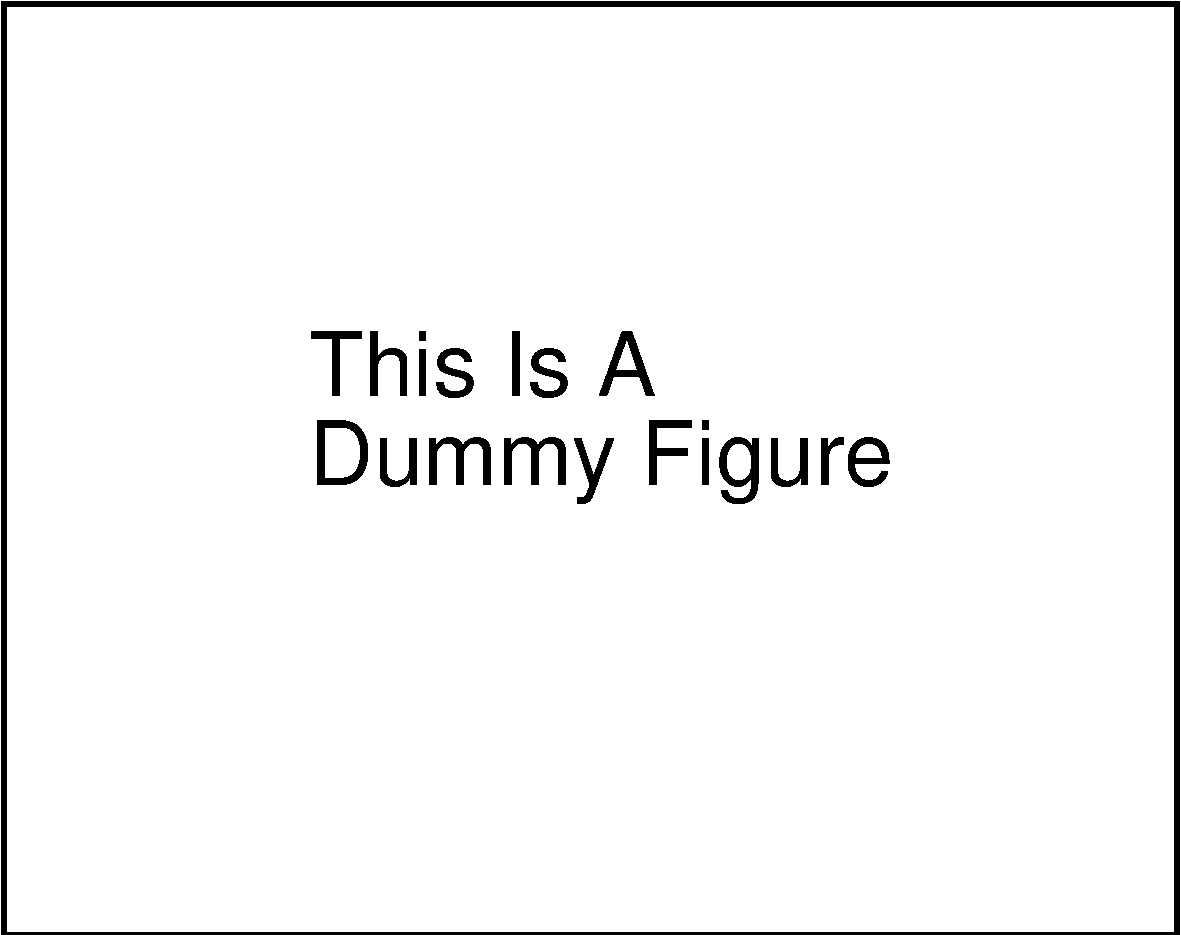
\includegraphics[width=0.5\textwidth]{graphics/dummy.pdf}
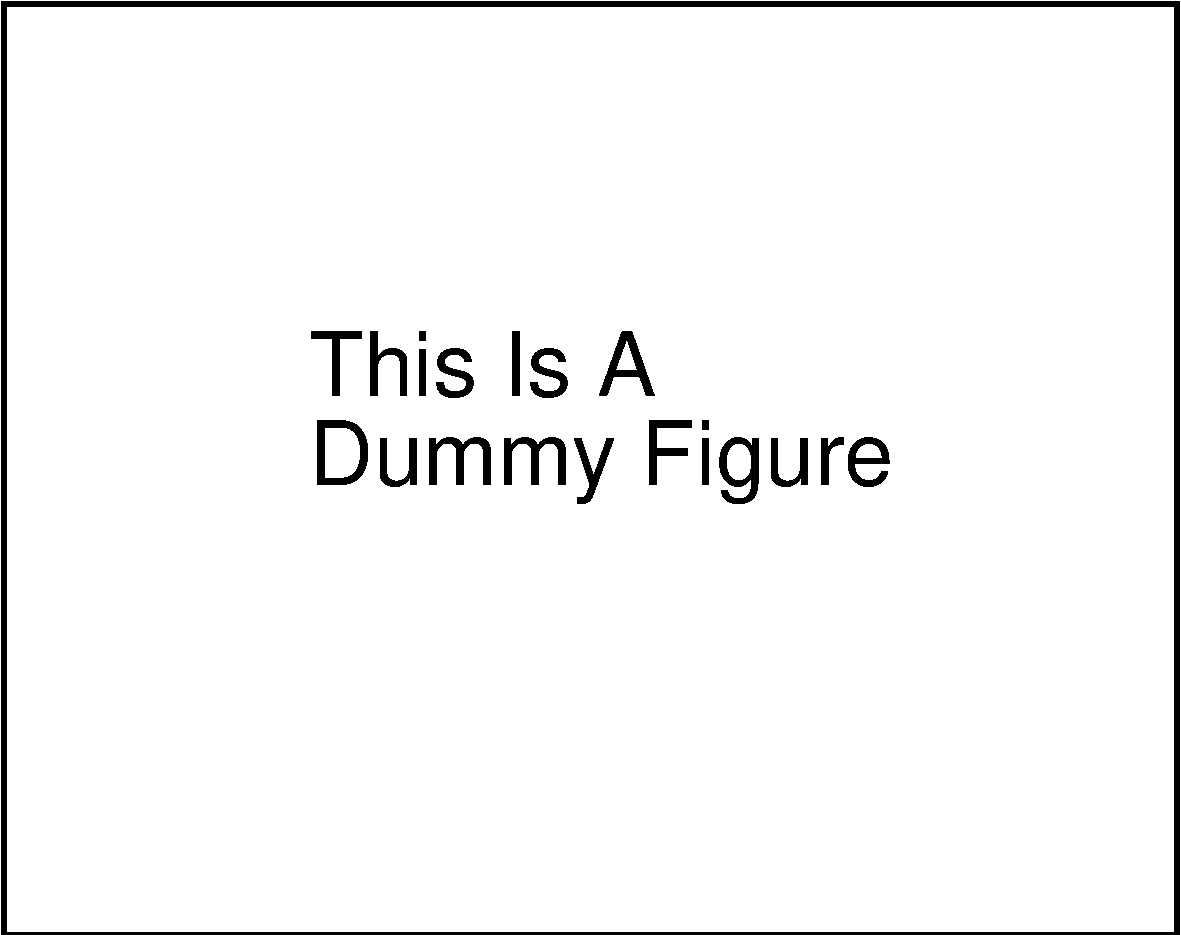
\includegraphics[width=0.5\textwidth]{graphics/dummy.pdf}}
\caption[Near detector constraints on heavy Majorana neutrinos]
{Upper limits on $U^2$, the mixing angle between heavy sterile
  neutrinos and the light active states, coming from the Baryon
  Asymmetry of the Universe (solid lines), from the seesaw mechanism
  (dotted line) and from the Big Bang nucleosynthesis (dotted
  line). The regions corresponding to different experimental searches
  are outlined by blue dashed lines. Left panel: normal hierarchy;
  right panel: inverted hierarchy (adopted
  from~\cite{Canetti:2010aw}).  Pink and red curves indicate the
  expected sensitivity of the DUNE near detector with an exposure of
  $5\times 10^{21}$ POT ($\sim 5$ years) with the \MWadj{1.2}
  reference beam at 120 GeV for detector lengths of \SI{7}{m} and
  \SI{30}{m} , respectively (see text for details).}
\label{fig:heavynu}
\end{figure}
%
It must be noted that exploitation of the complete 5 + 5 years ($\nu$ + $\overline\nu$) years 
of data taking would further improve the number of expected
events by a factor of  two, since it %this latter
scales linearly with the number of protons on target.  With the beam
upgrade to \SIadj{2.3}{MW}, this improvement would become a factor of
four with respect to the initial five year run and the %standard
\SI{1.2}{MW} beam.
A better sensitivity to $\nu$MSM can be achieved by instrumenting the
upstream region of the ND hall (e.g., with the liquid argon detector and some
minimal tracking device upstream). The fiducial volume of the new
detector will need to be empty (material-free) or fully sensitive in order
to suppress background events. The geometry of the ND hall would allow
a maximal decay length of about \SI{30}{m}. The sensitivity of this
configuration can be estimated by rescaling the expected limits on
the neutrino mixing angle $U^2$. The expected number of signal events with a total decay
length of $\sim30$~m exceeds by about 200 (800) times the number of
events in CHARM after a five (5 +5) year run with the standard (upgraded)
beam. In turn, this implies an improvement by a factor of 15 (28) in
the sensitivity to $U^2$ with respect to the CHARM experiment.
%It must be noted that i -------------   repetitive from 2 pgraphs up
If the magnetic moment of the sterile neutrinos
is sizeable, the dominant decay channel would be a radiative
electromagnetic decay into $\gamma \nu$, which has also been proposed
as a possible explanation for the observed MiniBooNE low-energy
excess~\cite{AguilarArevalo:2008rc}. This possibility,  in turn, requires a detector
capable of identifying and reconstructing single photon events.  The
low-density ND in DUNE can achieve an excellent 
sensitivity to this type of search as demonstrated by a similar analysis in
NOMAD~\cite{Kullenberg:2011rd}.
%%%%%%%%%%%%%%%%%%%%%%%%%%%%%%%%%%%%%%%%%%%%%%%
%\section{Search for High $\boldsymbol{\Delta m^2}$ Neutrino Oscillations}
\section{Search for High $\Delta m^2$ Neutrino Oscillations}
\fixme{removed bold. anne}
%\section{Search for Non-Standard Interactions: High $\Delta m^2$ Neutrino Oscillations}
\label{sec-high-delmsq}
The evidence for neutrino oscillations obtained from atmospheric,
long-baseline accelerator, solar and long-baseline reactor data from
different experiments consistently indicates two different scales,
with $\Delta m_{32}^2\sim$\SI{2.4e-3}{\eV^2} defining the
atmospheric oscillations (also long-baseline accelerator and
short-baseline reactor scales) and $\Delta m_{21}^2\sim$\SI{7.9e-5}{\eV^2} defining the solar oscillations (and long-baseline
reactor oscillations).  The only way to accommodate oscillations with
relatively high $\Delta m^2$ at the \si{\eV^2} scale as suggested by the
results from the LSND experiment~\cite{Volpe:2001qe} is therefore to
add one or more sterile 
neutrinos to the conventional three light
neutrinos.
Recently, the MiniBooNE experiment reported that its antineutrino
data might be consistent with the LSND $\overline{\nu}_\mu \to \overline{\nu}_e$
oscillation with $\Delta m^2\sim$ \si{\eV^2}~\cite{Maltoni:2007zf}.
Contrary to the antineutrino data, the %MiniBooNE 
neutrino data seem to
exclude high $\Delta m^2$ oscillations, possibly indicating a 
different behavior between neutrinos and antineutrinos.
Models with five (3+2) or six (3+3) neutrinos can potentially explain
the MiniBooNE results. In addition to the cluster of the three neutrino
mass states (accounting for \emph{solar} and \emph{atmospheric} mass splitting), two
(or three) states at the eV scale are added, with a small
admixture of $\nu_e$ and $\nu_\mu$ to account for the LSND signal. 
One distinct prediction from such models is a significant probability
for $\overline{\nu}_\mu$ disappearance into sterile neutrinos, on the order
of 10\%, in addition to the small probability for $\overline{\nu}_e$ appearance.

  Given a roughly \SIadj{500}{m} baseline and a low-energy beam, the DUNE ND
  can reach the same value $L/E_\nu$ as MiniBooNE and LSND. The
  large fluxes and the availability of fine-grained detectors make the
  DUNE program well suited to search for active-sterile neutrino
  oscillations beyond the three-flavor model with $\Delta m^2$ at the
  eV$^2$
  scale. 

Due to the potential differences between neutrinos and antineutrinos,
four possibilities have to be considered in the analysis: $\nu_\mu$
disappearance, $\overline{\nu}_\mu$ disappearance, $\nu_e$ appearance and
$\overline{\nu}_e$ appearance. As discussed in Section~\ref{sec-fluxosc},
the search for high $\Delta m^2$ oscillations has to be performed
simultaneously with the in situ determination of the fluxes.
To this end, an independent prediction of the $\nu_e$ and
$\overline{\nu}_e$ fluxes starting from the measured $\nu_\mu$ and $\overline{\nu}_\mu$ CC distributions are required since the $\nu_e$ and $\overline{\nu}_e$ CC distributions could
be distorted by the appearance signal. The low-$\nu_0$ method can provide
such predictions if external measurements for the $K_L^0$ component
are available from hadro-production experiments (Section~\ref{sec-fluxosc}). 
The study will implement an iterative procedure:
\begin{enumerate}%[parsep=-1pt]
\item extraction of the fluxes from $\nu_\mu$ and $\overline{\nu}_\mu$ CC distributions assuming
no oscillations are present
\item comparison with data and determination of oscillation parameters (if any)
\item new flux extraction after subtraction of the oscillation effect
\item iteration until convergence
\end{enumerate}
The analysis has to be performed separately for neutrinos and antineutrinos due to
potential CP or CPT violation, according to MiniBooNE/LSND data.
The ratio of $\nu_e$ CC events to $\nu_\mu$ CC events will be measured: 
\begin{equation}
{\mathcal{R}}_{e \mu} (L/E)  \equiv  \frac{\#~of~\nu_e N \to e^- X}{\#~of~\nu_\mu N \to \mu^- X }(L/E); \;\;\;\;\;\;\;  \overline{\mathcal{R}}_{e \mu} (L/E) \equiv \frac{\#~of~\overline{\nu}_e N \to e^+ X}{\#~of~\overline{\nu}_\mu N \to \mu^+ X }(L/E)
\end{equation}
This is then compared with the predictions obtained from the low-$\nu_0$ method.
Deviations of ${\mathcal{R}}_{e \mu}$ or $\overline{\mathcal{R}}_{e \mu}$ from the expectations
as a function of $L/E$ would provide evidence for oscillations. %It must be noted that t
This procedure only provides a relative measurement of $\nu_e (\overline{\nu}_e)$
versus $\nu_\mu (\overline{\nu}_\mu)$; since the fluxes
are extracted from the observed $\nu_\mu$ and $\overline{\nu}_\mu$ CC distributions, an analysis
of the ${\mathcal{R}}_{e \mu} (\overline{\mathcal{R}}_{e \mu})$ ratio cannot distinguish
between $\nu_\mu (\overline{\nu}_\mu)$ disappearance and $\nu_e (\overline{\nu}_e)$ appearance.
The process of NC elastic scattering off protons (Section~\ref{sec-deltas})
can provide the complementary measurement
needed to disentangle the two hypotheses of $\nu_\mu (\overline{\nu}_\mu)$ disappearance into
sterile neutrinos and $\nu_e (\overline{\nu}_e)$ appearance. In order to cancel systematic
uncertainties, the NC/CC ratio with respect to QE scattering will be measured:
\begin{equation}
{\mathcal{R}}_{NC} (L/E)  \equiv  \frac{\#~of~\nu p \to \nu p}{\#~of~\nu_\mu n \to \mu^- p }(L/E); \;\;\;\;\;\;\; \overline{\mathcal{R}}_{NC} (L/E) \equiv \frac{\#~of~\overline{\nu} p \to \overline{\nu} p}{\#~of~\overline{\nu}_\mu p \to \mu^+ n }(L/E)
\end{equation}
It is possible to reconstruct the neutrino energy from the proton
angle and momentum under the assumption that the nuclear smearing
effects are small enough to neglect (the same for the neutrino CC
sample). In the oscillation analysis, only the \emph{relative}
distortions of the ratio ${\mathcal{R}}_{NC}
(\overline{\mathcal{R}}_{NC})$ as a function of $L/E$ are of interest,
not their absolute values. For $Q^2>0.2$~GeV$^2$ the relative shape of
the total cross sections is not very sensitive to the details of the
form factors.  To improve the energy resolution, it is possible to use
neutrino interaction events originating from the deuterium inside the
D$_2$O target embedded into the fine-grained tracker. These events
have better energy resolution due to the smaller nuclear smearing
effects in D$_2$O.
An improved oscillation analysis is based on a simultaneous fit to
both ${\mathcal{R}}_{e \mu} (\overline{\mathcal{R}}_{e \mu})$ and
${\mathcal{R}}_{NC} (\overline{\mathcal{R}}_{NC})$. The first ratio
provides a measurement of the oscillation parameters while the latter
constrains the $\nu_e(\overline{\nu}_e)$ appearance versus the
$\nu_\mu(\overline{\nu}_\mu)$ disappearance. This analysis %results in
imposes two main requirements %for
on the ND:
\begin{itemize}%[parsep=-1pt]
\item $e^+/e^-$ separation to provide an unambiguous check of the different
behavior between neutrinos and antineutrinos suggested by MiniBooNE
\item accurate reconstruction of proton momentum and angle
\end{itemize}
Validation of the unfolding of the high $\Delta m^2$ oscillations from
the in situ extraction of the $\nu(\overline{\nu})$ flux would
also require changes to the beam conditions, since the ND cannot be
easily moved. This would require a short run with a high-energy beam
and the capability to change or switch off the beam focusing system.
%\fixme{It might be nice to have a summary??}
%   \subsection{The \nmne\ and \anmne\ Oscillation}   
%   \subsection{\nmnt\ and \nent\ Oscillation}   
%   \subsection{Non-Standard Interactions} 
%%%%%%%%%%%%%%%%%%%%%%%%%%%%%%%%%%%%%%%%%%%%%%%%%%%%%%
\section{Light (sub-GeV) Dark Matter Searches}
According to the latest cosmological and astrophysical measurements,
nearly eighty percent of the matter in the Universe is in the form of
cold, non-baryonic dark matter (DM)~\cite{Ade:2013zuv,Bennett:2012zja}. 
%\fixme{This is sort of common knowledge, but in a doc like this maybe should have a reference? Also, the 'non-baryonic' doesn't exclude electrons; is this an issue? RP: reference added, electron density is small and generally added to the baryonic}
The search to find evidence of the particle (or particles) that make
up DM, however, has so far turned up empty.  Direct detection
experiments and indirect measurements at the LHC, however, are
starting to severely constrain the parameter space of
Weakly-Interacting Massive Particles (WIMPs), one of the leading
candidates for DM.  The lack of evidence for WIMPs at these
experiments has forced many in the theory community to
reconsider.% the WIMP paradigm.
% AH split pgraph here -- too long
Some theories consider an alternative possibility to the WIMP paradigm
in which the DM mass is much lighter than the electroweak scale (e.g.,
below the GeV level). In order to satisfy constraints on the relic
density of DM, these theories require that DM particles be accompanied
by light \emph{mediator} particles that would have allowed for efficient
DM annihilation in the early Universe. In the simplest form of these
theories an extra U(1) gauge field mixes with the SM
U(1) gauge field, but with an additional kinetic term.  This mixing
term provides a \emph{portal} from the dark sector to the charged
particles of the SM.  In this model, the mediators are called \emph{dark
photons} and are denoted by $V$.
%\textit{\textbf{V}}.  % AH split pgraph here -- too long

  Recently, a great deal of interest has been paid to the possibility
  of studying models of light (sub-GeV) Dark Matter at low-energy,
  fixed-target
  experiments~\cite{Batell:2009di,deNiverville:2011it,deNiverville:2012ij,Dharmapalan:2012xp}.
  High-flux neutrino beam experiments --- such as DUNE --- have been
  shown to potentially provide coverage of DM+mediator parameter space
  that cannot be covered by either direct detection or collider
  experiments.

Upon striking the target, the proton beam can produce the dark photons
either directly through $pp(pn)\rightarrow {V}$ %\bf {V}$
as in the left-hand diagram of Figure~\ref{fig:dm} or indirectly
through the production of a $\pi^{0}$ or a $\eta$ meson which then
promptly decays into a SM photon and a dark photon as in the center
diagram in the figure. %Figure~\ref{fig:dm} (center).
For the case where $m_{V} > 2m_{DM}$, the dark photons will quickly
decay into a pair of DM particles.
%
\begin{figure}[!htb]
\centering
\tikzset{
  quark/.style={draw=blue, postaction={decorate},
    decoration={markings,mark=at position .5 with {\arrow[draw=blue]{>}}}},
  electron/.style={draw=pink, postaction={decorate},
    decoration={markings,mark=at position .5 with {\arrow[draw=blue]{>}}}},
  neutrino/.style={draw=red, postaction={decorate},
    decoration={markings,mark=at position .5 with {\arrow[draw=blue]{>}}}},
  heavy/.style={draw=red, dashed},
  pion/.style={draw=black,postaction={decorate},
    decoration={markings,mark=at position .5 with {\arrow[draw=blue]{>}}}},
  nucleus/.style={ultra thick, draw=black,postaction={decorate},
    decoration={markings,mark=at position .5 with {\arrow[draw=blue]{>}}}},
  muon/.style={draw=purple, postaction={decorate},
    decoration={markings,mark=at position .5 with {\arrow[draw=blue]{>}}}},
  gamma/.style={thick, decorate, decoration={snake,amplitude=3pt, segment length=6pt}, draw=red},
}
  \begin{minipage}[c]{0.3\textwidth}
    \begin{center}
\scalebox{0.60}{
\begin{tikzpicture}[ultra thick, node distance=2cm and 1.5cm]
\coordinate[] (center);
\coordinate[left=of center] (gam);
\coordinate[below left=of gam] (qm);
\coordinate[above left=of gam] (qp);
\coordinate[right=of center] (vee);
\coordinate[below right=of vee] (chid);
\coordinate[above right=of vee] (chi);
\draw[quark] (qp) -- node[below]{$q$} (gam);
\draw[quark] (gam) -- node[above]{$q$} (qm);
\draw[gamma] (gam) -- node[above]{$\gamma$} (center) node {$\bullet$};
\draw[gamma] (center) -- node[above]{V} (vee);
\draw[heavy] (vee) -- node[above]{$\chi$} (chi);
\draw[heavy] (vee) -- node[above]{$\chi^\dagger$} (chid);
\end{tikzpicture}
}
    \end{center}
  \end{minipage}
  \begin{minipage}[c]{0.3\textwidth}
    \begin{center}
\scalebox{0.60}{
\begin{tikzpicture}[ultra thick, node distance=1.4cm and 1.7cm]
\coordinate[] (center);
\coordinate[left=of center] (gamgam);
\coordinate[left=of gamgam] (mes);
\coordinate[above right=of gamgam,label=right:{$\gamma$}] (gam1);
\coordinate[below right=of gamgam] (gam2);
\coordinate[right=of gam2] (veedk);
\coordinate[above right=of veedk] (chi);
\coordinate[below right=of veedk] (chid);
\draw[pion] (mes) -- node[below]{$\pi^0,\eta$} (gamgam);
\draw[gamma] (gamgam) -- (gam1);
\draw[gamma] (gamgam) -- node[above]{$\gamma$}(gam2);
\draw[gamma] (gam2) -- node[above]{V} (veedk) node{$\bullet$};
\draw[heavy] (veedk) -- node[above]{$\chi$}(chi);
\draw[heavy] (veedk) -- node[above]{$\chi^\dagger$}(chid);
\end{tikzpicture}
}
    \end{center}
  \end{minipage}
  \begin{minipage}[c]{0.3\textwidth}
    \begin{center}
\scalebox{0.65}{
\begin{tikzpicture}[ultra thick, node distance=1cm and 1.5cm]
\coordinate[] (center);
\coordinate[above=of center] (chichi);
\coordinate[above left=of chichi] (chi1);
\coordinate[above right=of chichi] (chi2);
\coordinate[below=of center] (enen);
\coordinate[below left=of enen] (en1);
\coordinate[below right=of enen] (en2);
\draw[heavy] (chi1) -- node[below]{$\chi$} (chichi)  node{$\bullet$} -- node[below]{$\chi$} (chi2);
\draw[nucleus] (en1) -- node[above]{N} (enen);
\draw[nucleus] (enen)  node{$\bullet$} -- node[above]{N} (en2);
\draw[gamma] (chichi) -- node[left]{V} (center) node{$\bullet$};
\draw[gamma] (center) -- node[left]{$\gamma$} (enen);
\end{tikzpicture}
}
    \end{center}
  \end{minipage}
\caption[Production mechanisms for dark matter at neutrino-beam
experiments] {On the left is shown the direct production of a dark
  photon, while, in the center, the dark photon is produced via the
  decay of a neutral pion or eta meson. In both cases, the dark photon
  promptly decays into a pair of DM particles. Right: Tree-level
  scattering of a DM particle off of nuclei. Analogous interactions
  with electrons in the detector are also possible.}
\label{fig:dm}
\end{figure}
The DUNE ND together with the  high-intensity beam will provide an excellent setup for making this
measurement. The relativistic DM particles from the beam will travel along with
the neutrinos to the %DUNE near 
detector where they % The DM particles 
can  be detected through NC-like interactions either with
electrons or nucleons, % in the detector, 
as shown in the right-hand diagram of 
Figure~\ref{fig:dm}.  Since the signature of a DM event looks similar to that of
a neutrino event, the neutrino beam provides the major source of
background for the DM signal. % AH split pgraph here -- too long
Several ways have been proposed to suppress neutrino backgrounds using
the unique characteristics of the DM beam. Since DM will travel much
more slowly than the much lighter neutrinos, %with much higher masses,
DM events in the ND will arrive out of time with the %proton
beam pulse.
%
In addition, since the electrons struck by DM will be in a much more
forward direction compared to neutrino interactions, the angle of
these electrons may be used to reduce backgrounds, taking advantage of
the ND's fine angular resolution. % that DUNE can provide.
Finally, a special run can be devised to turn off the focusing horn to
significantly reduce the charged particle flux that will produce
neutrinos.  
Figure ~\ref{fig:wimp} shows the expected sensitivity of the MiniBooNE
DM search using this technique~\cite{Dharmapalan:2012xp}. With a
wider-band, higher-energy, more intense beam, DUNE is expected to not
only cover the MiniBooNE sensitivity region with higher statistics,
but will also extend the sensitivity to cover the region between 
MiniBooNE and the direct DM searches.
\begin{figure}[!tb]
\centerline{
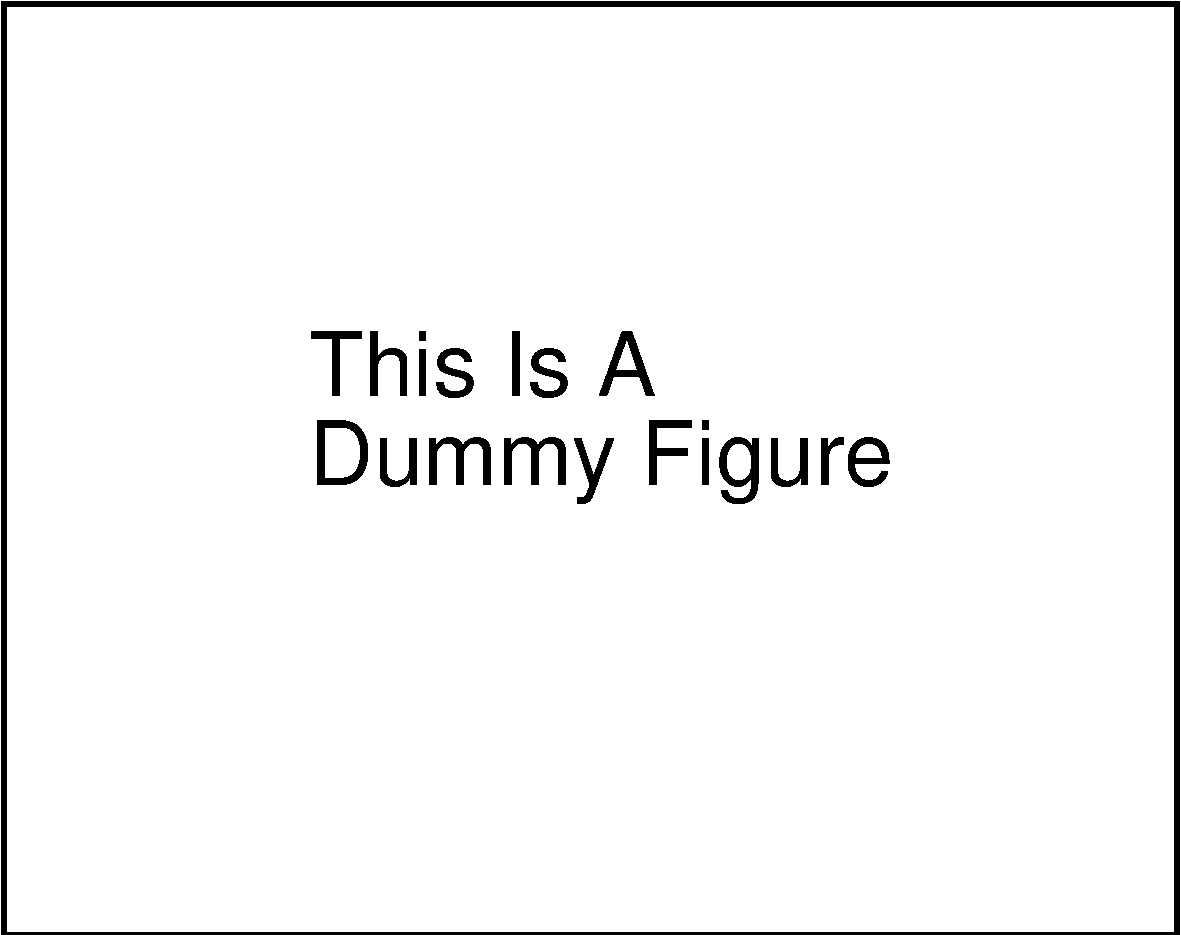
\includegraphics[width=\textwidth]{graphics/dummy.pdf}
}
\caption[Regions of nucleon-WIMP cross section versus WIMP
mass]{Regions of nucleon-WIMP scattering cross section (corresponding
  to dark matter in the lab moving with $v = 10^{-3}c$). The plot uses
  $m_V = 300$~MeV and $\alpha'=0.1$. Constraints are shown from
  different experiments.  The left plot shows the exclusion regions
  expected from MiniBooNE given 1-10 (light green), 10-1000 (green),
  and more than 1000 (dark green) elastic scattering events off
  nucleons. The right panel shows the same for elastic scattering off
  electrons. The magenta arrows indicate the region where DUNE can
  extend the MiniBooNE sensitivity. Figure is based on studies in ~\cite{Dharmapalan:2012xp}.}
\label{fig:wimp}
\end{figure}
If the DUNE ND were a LArTPC and the entire
detector volume active, the effective number of DM events detected
would be much higher when compared to a MINOS-like detector of the
same mass. Much more thorough studies must be conducted to obtain
reliable sensitivities. This requires an integration of theoretical
predictions into a simulation package for the detector.
% References for this section
% \bibitem{BATELL09} B. Batell, M. Pospelov and A. Ritz, ``Exploring Portals
%   to a Hidden Sector Through Fixed Targets,'' Phys. Rev. D 80,
%   095024 (2009), [arXiv:0906.5614 [hep-ph]].
% \bibitem{DENIVER11} P. deNiverville, M. Pospelov and A. Ritz,
%   ``Observing a light dark matter beam with neutrino experiments,''
%   Phys. Rev. D 84, 075020 (2011), [arXiv:1107.4580 [hep-ph]].
% \bibitem{DENIVER12} P deNiverville, D. McKeen and A. Ritz,
%   ``Signatures of sub-GeV dark matter beams at neutrino
%   experiments,'' Phys. Rev. D 86, 035022 (2012), [arXiv:1205.3499
%   [hep-ph]].
% \bibitem{DHARMAPALAN} R. Dharmapalan et al.  [MiniBooNE
%   Collaboration], ``Low Mass WIMP Searches with a Neutrino
%   Experiment: A Proposal for Further MiniBooNE Running,''
%   arXiv:1211.2258 [hep-ex].
% \bibitem{CERRILI05} M. Cirelli, N. Fornengo, T. Montaruli,
%   I. A. Sokalski, A. Strumia and F. Vissani, ``Spectra of neutrinos
%   from dark matter annihilations,'' Nucl. Phys. B 727, 99 (2005)
%   [Erratum-ibid. B 790, 338 (2008)], [hep-ph/0506298]
% \bibitem{AARTSEN13} M. G. Aartsen et al.  [IceCube Collaboration],
%   ``Search for dark matter annihilations in the Sun with the
%   79-string IceCube detector,'' Phys. Rev. Lett. 110, 131302
%   (2013)[arXiv:1212.4097 [astro-ph.HE]].

Figure~\ref{fig:es:NDhall} shows the current design of the underground hall required for the  \dword{nd} construction concept. The underground hall must house the detector components and allow required movement. The layout shows the space required for the detector, safety, and egress.  This  work is in progress. 


\begin{dunefigure}[DUNE near detector hall and detectors, plan view with dimensions]{fig:es:NDhall}
{\dword{dune}  \dword{nd} hall shown from above (top) and from the side transverse to the beam (bottom). The \dword{lartpc}, \dword{mpd}, and \dword{3dst} detectors are shown in position on the beam axis in both drawings.  On the top, the \dword{lartpc} is also shown in an off-axis position, suitable for module installation. }
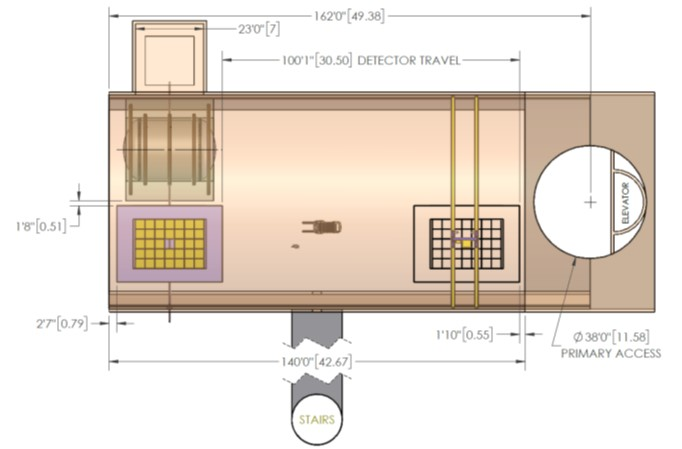
\includegraphics[width=0.8\textwidth]{graphics/NDhall1.jpg}
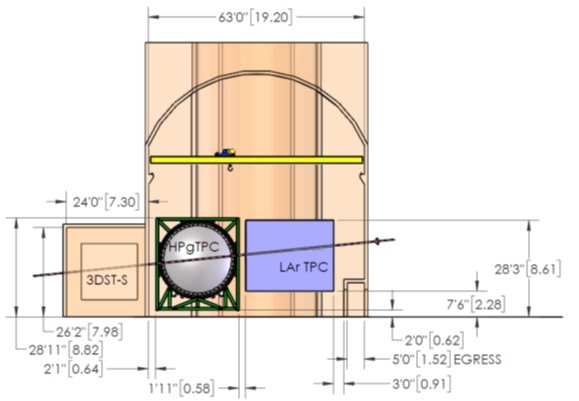
\includegraphics[width=0.8\textwidth]{graphics/NDhall2.jpg}
\end{dunefigure}

The overall construction method means the conventional facilities must meet certain requirements. 
The primary access shaft is large enough for lowering the pressure vessel and the magnet coils. The \dword{lar} cryostat is shown in its construction position near the main shaft. The \dword{mpd} and the \dword{lar} detector are also shown in the on-axis position. Because the \dword{3dst} detector does not need to move for \dword{duneprism}, it is shown in a dedicated alcove downstream of the \dword{lar} and multipurpose detectors.


The basic requirement for \dword{duneprism} is that both the \dword{mpd} and \dword{lar} detector can move horizontally to a position off the beam axis. The direction of the motion is to one side of the beam, and the total motion is approximately 30.5~m. 





